%----------------------------------------------------------------------------------------
%	PACKAGES AND OTHER DOCUMENT CONFIGURATIONS
%----------------------------------------------------------------------------------------

%\documentclass[12pt]{article}
\documentclass[a4paper,12pt,oneside]{book}

\usepackage[utf8]{inputenc}	% kódování textu
\usepackage[czech]{babel}		% zavedení češtiny
\usepackage[IL2]{fontenc}
\usepackage[pdftex]{hyperref}	% veškeré klikací odkazy
\usepackage{a4wide}
\usepackage{indentfirst}	% odsazení prvního řádku odstavce
\usepackage{amsmath,amsfonts,amssymb}	% matematika
\usepackage{graphicx}	% grafika
\usepackage{multirow}	% slouceni radek v tabulce
\usepackage{multicol}	% slouceni sloupcu v tabulce
\usepackage{longtable}	% rozdeleni tabulky pres vice stran
\usepackage{enumerate}	% seznamy
\usepackage{float}
\usepackage{booktabs}	% professional tables
\usepackage{lscape}		% stranka na sirku
\usepackage{fancyhdr}
\usepackage{url}
\usepackage{array}
\usepackage{wasysym}
\usepackage{listings} 
\usepackage{color}
\usepackage{caption}
\usepackage{subcaption}
\usepackage{dirtree}
\usepackage[subpreambles=true]{standalone}


\definecolor{light-gray}{gray}{0.97}

\newcommand{\latex}{\LaTeX}

\lstset{
numbers=left,
numberstyle=\tiny,
basicstyle=\ttfamily,
columns=flexible,
breaklines=true,
backgroundcolor=\color{light-gray},
xleftmargin=\parindent,
}

% % Define styles for lstlisting environment
\lstdefinestyle{python}{
   language=python,
   basicstyle={\ttfamily},
   keywordstyle=\color{blue}\ttfamily,
   stringstyle=\color{red}\ttfamily,
   commentstyle=\color{green}\ttfamily,
   showstringspaces=false,
   morekeywords={qDebug,QString,QgsVectorLayer,QgsMapLayerRegistry,QMessageBox,self}
}

\lstdefinestyle{sql}{
   language=sql,
   basicstyle={\ttfamily},
   keywordstyle=\color{blue}\ttfamily,
   stringstyle=\color{red}\ttfamily,
   commentstyle=\color{green}\ttfamily,
   showstringspaces=false,
   morekeywords={}
}

\lstdefinestyle{c++}{
   language=C++,
   basicstyle={\ttfamily},
   keywordstyle=\color{blue}\ttfamily,
   stringstyle=\color{red}\ttfamily,
   commentstyle=\color{green}\ttfamily,
   showstringspaces=false,
   morekeywords={AddInfo, EQUAL, QgsDebugMsg, QString, QgsVectorLayer, QList, QgsMapLayerRegistry}
}

\renewcommand\lstlistingname{Kód}
\renewcommand*{\lstlistlistingname}{Seznam ukázek kódu}

\usepackage[%
%top=40mm,
%bottom=35mm,
%left=40mm,
%right=30mm
top=40mm,
bottom=35mm,
left=35mm,
right=25mm
]{geometry}

% nastavení příkazu URL podle normy ISO
%\DeclareUrlCommand\url{\def\UrlLeft{< }\def\UrlRight{ >} \urlstyle{tt}}	% správné zobrazení www

\setlength{\parskip}{1ex}


\begin{document}
% ===============================================================
% NASTAVENI ZAHLAVI A ZAPATI	
% ===============================================================
% uvodni stranka zahlavi ani zapati mit nebude
\thispagestyle{empty}
 % vlevo text a název aktuální sekce
\lhead{
\includegraphics[scale=0.2]{images/cvut_logo.png}\hspace{10pt}ČVUT v~Praze}
 % vpravo název kapitoly
\rhead{{\rightmark}}

 % nastavime pouziti naseho stylu
\pagestyle{fancy}

\renewcommand{\chaptermark}[1]{\markright{#1}{}}
%\renewcommand{\sectionmark}[1]{\markright{#1}{}}

\fancypagestyle{plain}{
  \fancyhead{} % na prázdných stránkách nechci záhlaví
  \renewcommand{\headrulewidth}{0pt} % ani linku
}

% =========================
% TITULNÍ STRANA 11111111111
% =========================

\begin{titlepage}
 
\newcommand{\HRule}{\rule{\linewidth}{0.5mm}} % Defines a new command for the horizontal lines, change thickness here

\center % Center everything on the page

%----------------------------------------------------------------------------------------
%	HEADING SECTIONS
%----------------------------------------------------------------------------------------

\textsc{\LARGE České vysoké učení technické v~Praze}\\[0.5cm] % Name of your university/college
\textsc{\Large Fakulta stavební} % Major heading such as course name


%----------------------------------------------------------------------------------------
%	TITLE SECTION
%----------------------------------------------------------------------------------------

\vfill

\textsc{\LARGE Diplomová práce}

%----------------------------------------------------------------------------------------
%	AUTHOR SECTION
%----------------------------------------------------------------------------------------
\vfill
\begin{minipage}{0.4\textwidth}
\begin{flushleft} 
\large 2016	% datum
\end{flushleft}
\end{minipage}
~
\begin{minipage}{0.4\textwidth}
\begin{flushright} 
\large Bc. Štěpán \textsc{Bambula} \\ % Your name
\end{flushright}
\end{minipage}\\[1cm]

\end{titlepage}
% -------------------------------------------------------------------------------------------------------------


% =========================
% TITULNÍ STRANA 2222222222
% =========================

\begin{titlepage}
\center % Center everything on the page
 
%----------------------------------------------------------------------------------------
%	HEADING SECTIONS
%----------------------------------------------------------------------------------------

\textsc{\LARGE České vysoké učení technické v~Praze}\\[0.5cm] % Name of your university/college
\textsc{\Large Fakulta stavební}\\[0.5cm] % Major heading such as course name
\textsc{\large Studijní program: Geodézie a~kartografie}\\[0.5cm] % Minor heading such as course title
\textsc{\large Studijní obor: Geomatika}\\[0.5cm] % Minor heading such as course title

%----------------------------------------------------------------------------------------
%	LOGO SECTION
%----------------------------------------------------------------------------------------

\vspace{50pt}


\includegraphics[scale=1.2]{images/cvut_logo.png}  % Include a department/university logo 

%----------------------------------------------------------------------------------------
%	TITLE SECTION
%----------------------------------------------------------------------------------------

\vspace{40pt}

\textsc{\Large Diplomová práce}\\
\vfill
\textsc{\LARGE  Rozšíření nástroje pro práci s~katastrálními daty v~programu QGIS}\\[0.5cm] % Title of your document

\textsc{\Large QGIS VFK Plugin Improvements}
 
 
 %----------------------------------------------------------------------------------------
%	VEDOUCÍ PRÁCE
%----------------------------------------------------------------------------------------
 \vfill
\large Vedoucí práce: Ing. Martin \textsc{Landa}, Ph.D.

Katedra geomatiky
 
%----------------------------------------------------------------------------------------
%	AUTHOR SECTION
%----------------------------------------------------------------------------------------
\vfill
\begin{minipage}{0.4\textwidth}
\begin{flushleft} 
\large 2016	% datum
\end{flushleft}
\end{minipage}
~
\begin{minipage}{0.4\textwidth}
\begin{flushright} 
\large Bc. Štěpán \textsc{Bambula} \\ % Your name
\end{flushright}
\end{minipage}\\[1cm]
 
\end{titlepage}

%========================= ZADÁNÍ PRÁCE =================================
\clearpage
\pagestyle{empty}

\vspace*{\fill}
\begin{center}
\textsc{\Large Zde vložit zadání práce!!!}
\end{center}

\vspace*{\fill}

%========================= ABSTRAKT =====================================
\clearpage

\hfill

\noindent
\textsc{\Large Abstrakt}

\vspace{12pt}

Diplomová práce rozšiřuje stávající projekt laboratoře OSGeoREL ČVUT
v~Pra\-ze, který je zaměřen na práci s~katastrálními daty
poskytovanými ve výměnném formátu VFK v~prostředí open source nástroje
QGIS. Práce tento projekt, který je v~QGIS implementován jako
tzv. zásuvný modul, doplňuje o~novou funkcionalitu, kterou je
zpracování a~vizualizace datových změnových vět VFK. S~tímto souvisí
i~nezbytné změny na straně ovladače VFK v~knihovně GDAL, který zásuvný
modul pro čtení dat používá. Druhotným cílem diplomové práce je
usnadnění distribuce zásuvného modulu, což souvisí s~přepisem
stávajícího projektu do jazyka Python.


\vspace{32pt}

\noindent
\textsc{\Large Klíčová slova}

\vspace{12pt}

VFK, NVF, QGIS, ISKN, Python, PyQt, GDAL, zásuvný modul


\vfill

\noindent
\textsc{\Large Abstract}

\vspace{12pt}

Diploma thesis extends the existing project of OSGeoREL at the Czech
Technical University in Prague which is focused on working with the
cadastral data provided in exchange format VFK in an environment of
open source software QGIS. The project which is implemented in QGIS as
a~so-called plugin is in this thesis extended with new functionality
-- processing and visualisation of amendment records of VFK. It is
related to the necessary changes of the VFK driver in GDAL library
which plugin uses for reading data. Another goal of this study is to
facilitate the distribution of plugin which is related to a~transcript
of an existing project to Python programming language.

\vspace{32pt}

\noindent
\textsc{\Large Keywords}

\vspace{12pt}
VFK, NVF, QGIS, ISKN, Python, PyQt, GDAL, plugin


\vfill

%========================= PROHLÁŠENÍ ==================================
\clearpage
\vspace*{\fill}

\noindent
\textsc{\Large Prohlášení}

\vspace{12pt} Prohlašuji, že jsem diplomovou práci na téma
\uv{Rozšíření nástroje pro práci s~katastrálními daty v~programu QGIS}
vypracoval samostatně. Všechny podklady, ze kterých jsem čerpal, jsou
uvedeny v~seznamu použité literatury.

\vspace{24pt}
\noindent
\begin{minipage}{0.4\textwidth}
\begin{flushleft}
\center 
V~Praze dne \dots \dots \dots \\
\end{flushleft}
\end{minipage}
~
\begin{minipage}{0.8\textwidth}
\begin{flushright} 
\vspace{20pt}
\center
\dots \dots \dots \dots \dots \dots \dots \dots \\
Štěpán Bambula
\end{flushright}
\end{minipage}\\[2cm]


%========================= PODĚKOVÁNÍ ==================================
\clearpage
\vspace*{\fill}

\noindent
\textsc{\Large Poděkování}

\vspace{12pt} Na tomto místě bych chtěl poděkovat vedoucímu diplomové
práce Ing. Martinu Landovi, PhD. za pomoc, připomínky a~poskytnuté
rady při zpracování této práce. Dále bych chtěl poděkovat Jiřímu
Chroustovi za rady ohledně zpracování změnových vět. V~neposlední řadě
děkuji rodině za podporu během celého studia.  \vspace{2cm}

%======================POUZITE ZKRATKY===============================
\clearpage
%\rhead{SEZNAM POUŽITÝCH ZKRATEK}		 % vpravo název kapitoly
\chapter*{Seznam použitých zkratek}
\thispagestyle{empty}

\begin{description}
\item[VFK] Výměnný formát katastru nemovitostí
\item[NVF] Nový výměnný formát
\item[ČUZK] Český úřad zeměměřický a~katastrální
\item[GDAL] Geospatial Data Abstraction Library
\item[GIS] Geografický informační systém
\item[OSGeo] Open Source Geospatial Foundation
\item[ISKN] Informační systém katastru nemovitostí
\item[SGI] Soubor geodetických informací
\item[SPI] Soubor popisných informací
\item[API] Application Programming Interface
\end{description}


%=========================OBSAH=======================================
\clearpage
\rhead{{\rightmark}}		% vpravo název kapitoly
\tableofcontents
\thispagestyle{empty}

%============================ÚVOD====================================
\clearpage
\pagestyle{fancy}		% nastaví styl stránky a číslování
\setcounter{page}{1}   	% nastaví čítač stránek znovu od jedné
\pagenumbering{arabic} % číslování arabskými
\rhead{Úvod}		 % vpravo název kapitoly
\chapter*{Úvod}
\addcontentsline{toc}{chapter}{Úvod}

Katastr nemovitostí je, co se týče objemu uchovávaných dat, jedním
z~nejrozsáhlejších informačních systémů ve státní správě. Proto i~jeho
data jsou velice zajímavým zdrojem informací ať už pro uživatele ze
státní sféry, či pro společnosti zabývající se například územním
plánováním. Vzhledem k~tomu, že data obsahují nejen popisnou, ale
i~prostorovou složku, tak na nich může být prováděno široké spektrum
prostorových analýz.

%%% ML: techto dat, nize v textu mas VFK bez blizsiho vysvetlene (data
%%% KN jsou poskytovana ve Vymennem formatu ...)
Pro zpracování těchto dat je k~dispozici několik nástrojů. Většinou se
však jedná o~komerční nástroje, které jsou šířeny za úplatu, nebo
o~nástroje, které jsou dostupné jako modul pro komerční GIS software
%%% ML: Kokes a dalsi
typu ArcGIS nebo AutoCAD Map 3D.

Výsadní postavení placených programů pro práci s~geografickými daty se
%%% ML: o nabourani nejde, ani o to, ze je zdarma ;-)
v~posledních letech snaží nabourat projekt QGIS, který je šířen zdarma
%%% ML: licence open source neexistuje, zmeneno
jako open-source. To se mu daří i~díky mnoha dobrovolníkům,
kteří se na jeho vývoji podílí. Nemalý podíl na úspěchu tohoto
open-source programu má i~knihovna GDAL, díky které je QGIS schopen
číst, či zapisovat do širokého spektra vektorových, ale i~rastrových
formátů.

%%% ML: dvakrat ovladac ve vete, zmenoveno na soucast, nic lepsiho me nanapadlo
Pro Českou republiku je jednou z~nejdůležitějších součástí knihovny
GDAL ovladač VFK, který podporuje čtení právě ze souborů
vyexportovaných z~Informačního systému katastru nemovitostí
v~tzv. novém výměnném formátu (VFK). Spolu s~vývojem knihovny GDAL se
vyvíjí i~samotný ovladač a~od své první verze v~roce 2011 byl obohacen
o~spoustu nových funkcionalit. Jednou z~nich je například podpora
čtení z~databáze SQLite, vznikající při čtení dat VFK knihovnou
GDAL. Tato funkcionalita byla přidána i~díky této diplomové práci.

Pro usnadnění práce s~daty ve výměnném formátu katastru nemovitostí
v~prostředí QGIS vznikl na Fakultě stavební ČVUT v~Praze roku 2012
zásuvný modul, jehož autory jsou absolventi oboru
Geoinformatika Anna Kratochvílová a~Václav Petráš. Tento modul byl
napsán v~jazyce C++ a~obsahoval široké spektrum nástrojů, díky kterým
bylo možné soubory VFK načíst, zobrazit v~mapovém okně QGIS a~provádět
nad nimi vyhledávací dotazy, včetně možnosti exportu výsledků do
některého z~podporovaných formátů.

%%% ML: zkus pouzit jine slovo nez slabina
Největší slabinou tohoto nástroje byl paradoxně použitý jazyk C++,
díky čemuž byla instalace a~zprovoznění zásuvného modulu v~QGIS ne
zcela intuitivní a~pro běžného uživatele mnohdy představovala
%%% ML: v textu mas casto "toto", tohoto, zkus se tomu vyhnout
nepřekonatelný problém. Na základě tohoto podnětu vzniklo jedno
z~podtémat této diplomové práce, a~to přepis stávajícího zásuvného
%%% ML: nasjedujici vetu preformulovat, nezni cesky
modulu do jazyka Python. Tento jazyk byl zvolen z~důvodu, protože QGIS
podporuje zásuvné moduly napsané právě v~těchto dvou jazycích. Oproti
%%% ML: spojit dve nasledujici vety do jedne, zkratit
modulům napsaným v~jazyce C++ mají moduly v~jazyce Python výhodu
snadné instalace v~prostředí QGIS. Takto napsané moduly jsou v~QGIS
dostupné standardní cestou, čili ze správce zásuvných modulů.

%%% ML: ich forma v uvodu je akceptovatelna, jinak se pouziva "my",
%%% tj. zamerime a pod.
V~teoretické části diplomové práce se zaměřím na nezbytnou rešerši
nástrojů, které mohou být pro zpracování katastrálních dat
použity. Uvedu zde zástupce jak z~komerční sféry, tak nástroje, které
jsou dostupné bezúplatně -- především tedy výše zmíněný ovladač VFK
knihovny GDAL. V~další kapitole teoretické části se budu věnovat
popisu použitých technologií, bez kterých by diplomová práce nemohla
být zpracována.

V~posledních dvou částech teoretického úvodu se budu věnovat
Informačnímu systému katastru nemovitostí, jež je zdrojem dat ve
formátu VFK, a~popisu výměnného formátu. Při popisu formátu budu
čerpat především z~oficiální dokumentace, která je k~němu dostupná
s~tím, že zde uvedu pouze nezbytné informace k~pochopení struktury, do
které jsou data exportována. Samozřejmě zde popíši i~uchování
a~strukturu změnových vět, jejichž zpracování je nosným tématem
diplomové práce.

V~praktické části nejprve přiblížím stávající zásuvný modul napsaný
v~jazyce C++, kde se zaměřím na jeho instalaci v~prostředí QGIS
a~především na jeho funkcionalitu. Po této kapitole plynule naváži na
rozšíření stávající funkcionality. Zde budou nejprve uvedeny kroky
související s~usnadněním distribuce modulu. Kapitola bude pokračovat
změnami, které musely být provedeny na straně ovladače VFK knihovny
GDAL tak, aby byl zásuvný modul schopen číst a~zpracovávat změnové
věty výměnného formátu. O~implementaci zpracování změnových vět
pojednává dal\-ší část kapitoly. Poslední podkapitolou praktické části
bude popis jednotlivých tříd zásuvného modulu tak, aby mohl kdokoliv
na tuto diplomovou práci navázat.

Výstupem práce tedy bude přepsaný zásuvný modul do programovacího
jazyka Python, který bude doplněn o~nové funkcionality. Jednou
z~nejdůležitějších bude zpracování změnových vět výměnného formátu
a~jejich aplikace na stavová data uložena v~databázi SQLite.


% =============================================================================
\clearpage
\rhead{{\rightmark}}
\chapter{Rešerše nástrojů pro práci s~VFK}

V~současné době existuje několik nástrojů pro práci s~katastrálními
daty. Ať už se jedná o~moduly, které jsou distribuovány zdarma, nebo
za úplatu, jako nadstavba pro komerční nástroje, případně o~moduly
dostupné pro open-source nástroje. S~trochou nadsázky se dá říci, že
%%% ML: vetsi software zni divne
každý větší software pro práci s~prostorovými daty má svůj zásuvný
modul (nadstavbu) pro práci s~daty \textit{VFK}.

%%% ML: Ich forma se v textu prace nepouziva (nemela by se pouzivat),
%%% maximalne v uvodu a zaveru, tj. se budeme věnovat, zmenit to v
%%% celem textu bude narocne a zaneses tam radu chyb, pokud to mas v
%%% celem textu, tak navrhuji asi nechat
V~této kapitole bych se chtěl věnovat vybraným nástrojům pracujícím
s~těmito daty. Moduly, které jsou šířeny zdarma a~bylo je možné
vyzkoušet, byly otestovány přímo. Popis komerčních modulů vychází
především z~dostupně dokumentace na příslušných oficiálních webových
stránkách.

\section{ISKN Studio pro ArcGIS}
\label{l_iskn_studio}
% TODO: https://www.arcdata.cz/produkty/ceska-specifika/iskn-pro-arcgis-for-desktop
Aplikace ISKN Studio slouží pro převod dat VFK do ESRI geodatabáze, se
kterou je schopen pracovat program ArcGIS. Struktura geodatabáze je
navržena dle připravené šablony. Tato šablona je vždy vázána k~dané
verzi formátu VFK a~může být stažena přímo ze stránek společnosti
Arcdata Praha, která je zároveň tvůrcem této aplikace. Data načtená
touto aplikací mohou být exportována také ve formátu
\textit{XML}. Díky této aplikaci může být v~geodatabázi sestavena
geometrie vektorových prvků. \cite{iskn_studio}

\begin{figure}[htb]
\centering
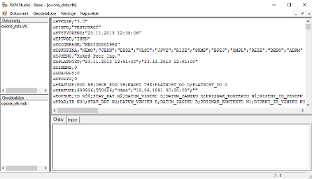
\includegraphics[width=.8\textwidth]{images/ISKNStudio-aplikace.png}
\caption[Aplikace ISKN Studio]{Aplikace ISKN Studio (zdroj: vlastní)}
\end{figure}

Strutura vytvořené geodatabáze je shodná s~datovými bloky obsaženými
ve vstupním souboru VFK (pro každý datový blok je vytvořena jedna
tabulka).

Aplikace disponuje kromě zpracování souboru VFK dalšími
funkcionalitami. Jednou z~hlavních je možnost kontroly struktury
vstupního VFK souboru podle zvolené šablony nebo podle
geodatabáze. Samozřejmostí je možnost uložení protokolu
%%% ML: vsechny jeji verze, nebo pouze ta zakladni?
o~zpracování. Aplikace je distribuována zdarma.

\newpage
\subsection{ISKN View pro ArcGIS}
% TODO: https://www.arcdata.cz/produkty/ceska-specifika/iskn-pro-arcgis-for-desktop
ISKN View je sesterskou aplikací ke zvýše zmíněnému ISKN Studio
(\ref{l_iskn_studio}). Software je používán jako doplněk
(\textit{Add-In}) v~programu ArcGIS verze 10.1 a~vyšší.

\begin{figure}[htb]
\centering
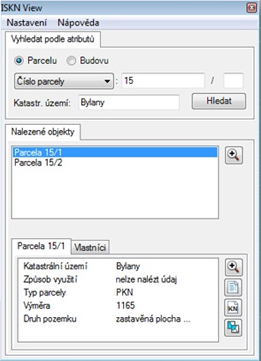
\includegraphics[scale=0.47]{images/ISKNView-aplikace.png}
\caption[Aplikace ISKN View]{Aplikace ISKN View (zdroj: \cite{iskn_studio})}
\end{figure}

Díky ISKN View je umožněno rychlé a~jednoduché vyhledávání v~datech
ISKN, která byla pomocí aplikace ISKN Studio převedena do některé
%%% ML: ted najednou pises o vice formatech (co podporuje krome File Geodatabaze?)
z~podporovaných geodatabází.  Aplikace je rovněž šířena
%%% ML: vsechny verze?
bezúplatně. \cite{iskn_studio}

\newpage
\section{Import dat KN ve výměnném formátu}
%%% ML: nastoj ma opravdu tak obecny nazev?
% TODO: http://www.gisoft.cz/Moduly/ImportVFK
Jedná se o~modul vytvořený společností GISOFT, který slouží k~převodu
a~načtení dat ve formátech VFK a~VKM do formátu DGN. Modul
spolupracuje s~produkty společnosti Bentley Systems, především
MicroStation. Umožňuje načtení dat jak ve starém, tak i~v~novém
výměnném formátu (viz kapitola č. \ref{l_format_vfk}) KN. Je dostupný
jako volitelný modul pro nadstavby
\textbf{MGEO}\footnote{\url{http://www.gisoft.cz/MGEO/MGEO}}
a~\textbf{SPIDER}\footnote{\url{http://www.gisoft.cz/SPIDER/SPIDER}}. Může
být použit v~následujících případech:

\begin{description}
\item[Samostatně:] Použití samostatně se hodí v~případě, kdy jsou
  načítána data výměnného formátu obsahující pouze katastrální
  mapu. V~tomto případě bude vstupní soubor převeden do podoby výkresu
  ve formátu DGN.

\item[Spolu s~modulem Práce s~popisnými informacemi KN:] Tento mód je
  užiteč\-ný v~případě, kdy jsou v~souboru spolu s~katastrání mapou
  dostupné i~popisné informace (případně jsou uvedeny pouze popisné
  informace).
\end{description}

\begin{figure}[htb]
\centering
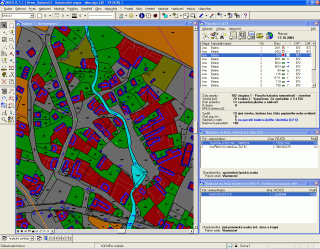
\includegraphics[scale=1]{images/microstation_modul.png}
\caption[Import dat KN ve výměnném formátu -- ukázka použití]{Import dat KN ve výměnném formátu -- ukázka použití (zdroj: \cite{gisoft_modul})}
\end{figure}

Veškeré informace uvedené o~tomto modulu vycházejí z~oficiálního
popisu modulu uvedeného na stránkách společnostu
GISOFT. \cite{gisoft_modul}

\newpage
\section{Spirit VFK}
% TODO: http://www.georeal.cz/cz/spirit-desktop/spirit-vfk
Software Spirit VFK je vytvořen a~distribuován společností GEOREAL
jako samostatně spustitelná desktopová aplikace. Slouží pro převod dat
(VFK) katastru nemovitostí do jakékoli geodatabáze podporované
společností ESRI.

Do geodatabáze jsou postupně importovány tabulky, relace a~ostatní
obsažené objekty ISKN. Takto vytvořená databáze může být použita
v~souvisejících aplikačních nadstavbách \textbf{Spirit
  KN}\footnote{\url{http://www.georeal.cz/cz/spirit-desktop/spirit-kn}}
a~\textbf{Spirit Portál -
  KN}\footnote{\url{http://www.georeal.cz/cz/spirit-server/portal-kn}},
případně může sloužit pro další analytické práce nad daty KN. Import
dat do geodatabáze probíhá v~následujících krocích:

\begin{enumerate}
 \item příprava geodatabáze (tvorba tabulek, relací, \dots),
 \item import dat VFK,
 \item vektorizace parcel, budov a~ostatních mapových vrstev,
 \item optimalizace mapových vrstev, tvorba symbologie.
\end{enumerate}

Symbologie (ve formátech MXD a~LYR) vytvářená v~posledním kroku se
používá pro zobrazování dat ve výše zmíněných aplikačních nadstavbách
pro ArcMap. Aplikace Spirit VFK může být využívána pro pravidelnou
aktualizaci datových skladů katastru nemovitostí.

\begin{figure}[htb]
\centering
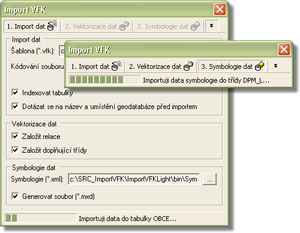
\includegraphics[scale=0.7]{images/spirit_vfk.png}
\caption[Spirit VFK -- ukázka aplikace]{Spirit VFK -- ukázka aplikace (zdroj: \cite{spirit_vfk})}
\end{figure}

Pro aplikaci existuje i~její odlehčená verze Spirit VFK Light, díky
které je možné importovat data VFK do osobní geodatabáze ArcGIS (MS
Access) nebo databáze MS SQL Server. Používání obou aplikací
nevyžaduje znalost struktury dat ISKN nebo výměnného formátu VFK.

Veškeré výše uvedené informace pocházejí z~oficiálních stránek
produktu, viz \cite{spirit_vfk}.

\section{VFK2DWG}
\label{l_vfk2dwg}
% TODO: http://www.cadstudio.cz/vfk2dwg
Jedná se o~aplikaci od společnosti CAD Studio. Slouží jako nadstavba
(utilita) pro produkty firmy Autodesk založených na AutoCadu (AutoCAD,
AutoCAD Architecture, AutoCAD Map 3D, AutoCAD Civil 3D, \dots). Díky
této aplikaci je možné do výše uvedených programů načíst data VF ISKN
(\textit{.vfk}) a~dále s~nimi pracovat.

\begin{figure}[htb]
\centering
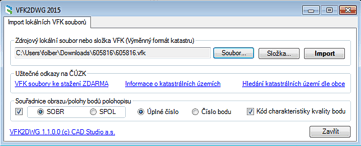
\includegraphics[scale=0.85]{images/vfk2dwg-aplikace.png}
\caption[Aplikace VFK2DWG]{Aplikace VFK2DWG (zdroj: \cite{cadstudio-vfk2dwg})}
\end{figure}

Aplikace převádí \textit{VFK} soubory na objekty (hranice parcel,
parcelní čísla, vnitřní kresby, popisy, \dots), se kterými je AutoCAD
schopen pracovat. Tyto objekty jsou pomocí hypertextových odkazů
provázány se stránkami ČUZK (respektive s~aplikací \textbf{Nahlížení
  do KN}), kde o~nich mohou být zjištěny dodatečné informace.

% \begin{figure}[htb]
% \centering
% 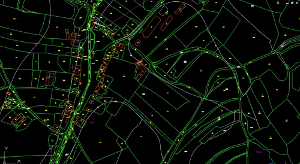
\includegraphics[width=\textwidth]{images/vfk2dwg-ukazka.png}
% \caption[Aplikace VFK2DWG -- ukázka načtených dat]{Aplikace VFK2DWG -- ukázka načtených dat (zdroj: \cite{cadstudio-vfk2dwg})}
% \end{figure}

Nejnovější verze aplikace pracuje i~s~daty formátu ve verzi 5.1 a~je
podporována i~v~AutoCAD 2016. Bohužel se jedná o~komerční aplikaci
a~proto nemohla být otestována. Veškeré informace byly převzaty
z~oficiálních stránek společnosti CAD Studio, viz
\cite{cadstudio-vfk2dwg}.


\section{VFK2DB}
% TODO: http://www.cadstudio.cz/vfk
VFK2DB je databázová varianta výše zmíněné aplikace (\ref{l_vfk2dwg}),
která se chová jako samostatně spustitelný program nezávislý na
konkrétním programu GIS či CAD.

Aplikace importuje data z~formátu \textit{VFK} do relační databáze
Oracle nebo MS SQL Server (v~budoucnu se počítá s~doplněním exportu do
dalších typů databází, např. PostGIS, SQLite). Takto vytvořená
databáze může být načtena některým z~GIS produktů založených na
prostorových SQL databázích (AutoCAD Map 3D, ESRI, Bentley,
Intergraph, GeoServer, MapServer, \dots).

Opět se jedná o~komerční aplikaci společnosti CAD Studio, a~proto
nemohla být otestována. Veškerý zde uvedený popis vychází z~oficiální
dokumentace na stránkách společnosti, viz \cite{cadstudio-vfk2db}.

\section{Topol VFK Import}
% TODO: http://www.datasystem.cz/vfk-import-s-37-m-4.html
Jak už ze samotného názvu plyne, aplikace Topol VFK Import byla
vyvinuta společností Data System s.r.o. ve spolupráci se společností
Topol Software. Aplikace disponuje vlastním grafickým prostředím, ve
kterém je možné VFK data exportovat do formátů DWG a~DXF, případně do
vlastního formátu (OpenGIS MDB) společnosti Topol.

Opět se jedná o~komerční aplikaci, a~proto nemohla být
vykoušena. Veškeré informace pocházejí z~webových stránek výrobce, viz
\cite{topol_vfk_import}.

\begin{figure}[htb]
\centering
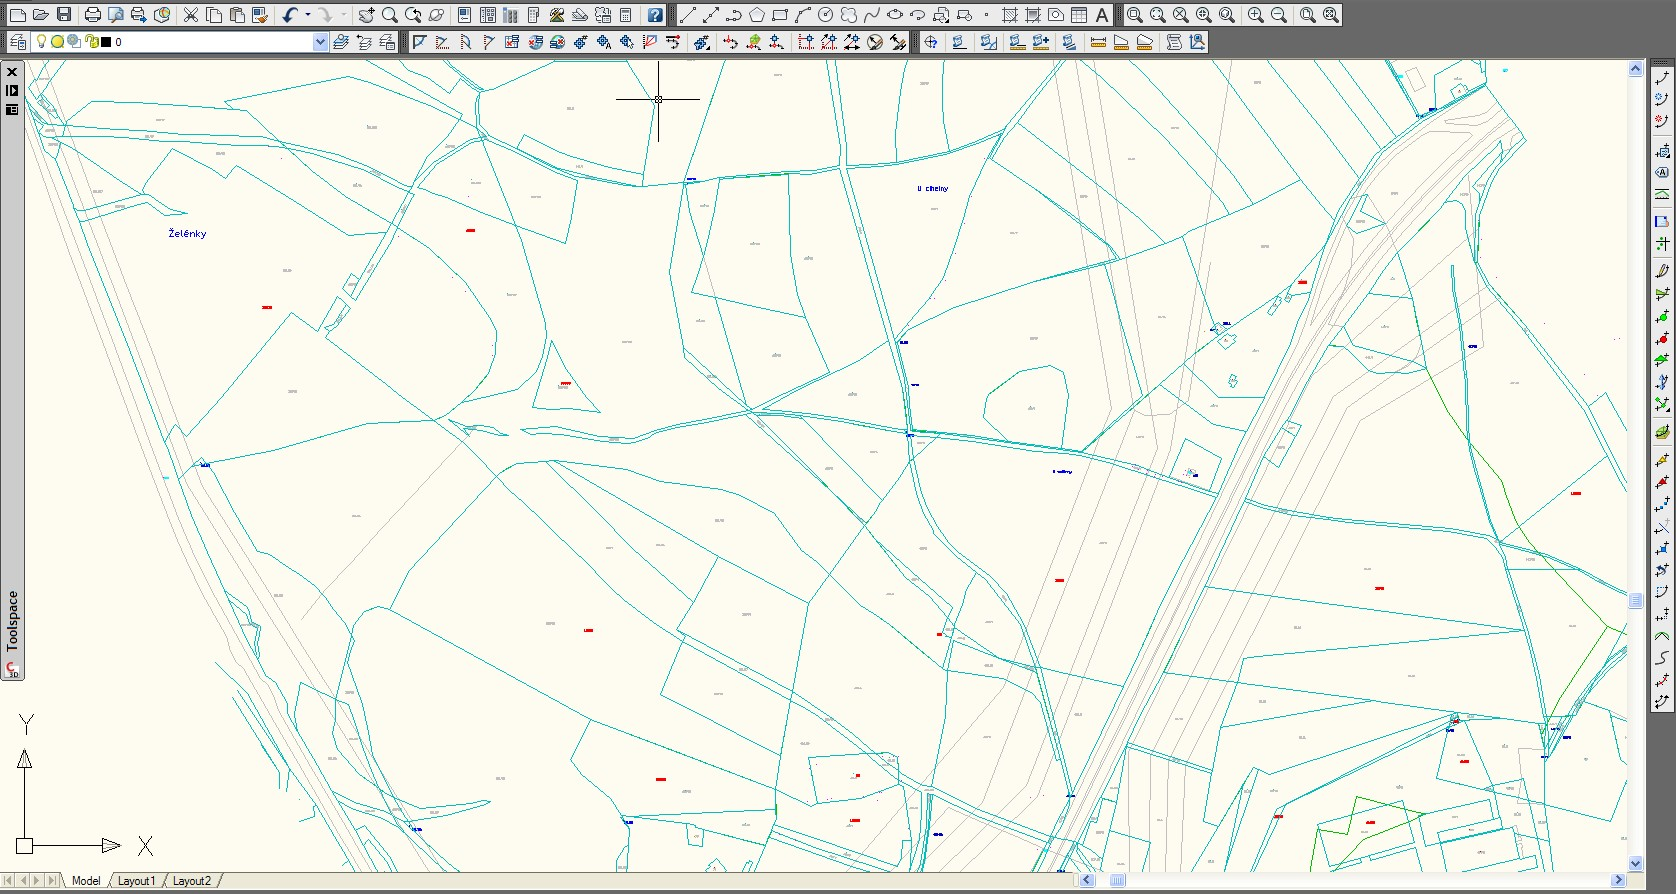
\includegraphics[width=\textwidth]{images/topol-aplikace.png}
\caption[Topol VFK Import -- ukázka zpracovaných dat]{Topol VFK Import -- ukázka zpracovaných dat (zdroj: \cite{topol_vfk_import})}
\end{figure}

\newpage
\section{GDAL -- VFK Driver}
% TODO: http://freegis.fsv.cvut.cz/gwiki/VFK_/_GDAL
% TODO: http://www.gdal.org/drv_vfk.html
% TODO: http://gama.fsv.cvut.cz/~landa/publications/2010/gis-ostrava-2010/paper/landa-ogr-vfk.pdf
VFK Driver, díky kterému je možné data VFK číst, je součástí knihovny
GDAL (viz \ref{l_gdal}) od verze 1.7. Vstupní VFK soubor je knihovnou
GDAL rozeznán jako \texttt{OGR datasource}, každý datový blok je poté
vnímán jako \texttt{OGR layer}. Od GDAL verze 1.10 je podpora VFK
přidána pouze v~případě, kdy je knihovna kompilována s~podporou SQLite
(\texttt{./configure --with-sqlite}).

Driver si interně data při prvním čtení ukládá do databáze SQLite ve
stejném adresáři, jako je umístěn VFK soubor. Při opětovném čtení
driver používá pro čtení již vytvořenou databázi. Tímto se opakované
načítání dat několikanásobně urychlí, viz porovnání níže. Implicitní
chování driveru může být ovlivněno zadáním proměnných prostředí.

\begin{multicols}{2}
\begin{lstlisting}
# prvni cteni
real	0m11.547s
user	0m11.016s
sys	0m0.232s
\end{lstlisting}
\columnbreak
\begin{lstlisting}
# opakovane cteni
real	0m0.317s
user	0m0.284s
sys	0m0.028s
\end{lstlisting}
\end{multicols}

Jednou z~nejdůležitějších je proměnná \texttt{OGR\_VFK\_DB\_NAME}
sloužící pro definici jména SQLite databáze. Neméně důležitá proměnná
\texttt{OGR\_VFK\_DB\_OVERWRITE} říká, že při každém čtení souboru VFK
se vytváří databáze SQLite znovu, čtení tedy probíhá pouze ze
souboru VFK. Níže je uvedena ukázka otevření souboru VFK. \cite{gdal_vfk}

\begin{lstlisting}[language=bash, showstringspaces=false, escapeinside={(*@}{@*)}]
$ ogrinfo Export_vse.vfk
Had to open data source read-only.
INFO: Open of `Export_vse.vfk'
      using driver `VFK' successful.
1: PAR (Polygon)
2: BUD (Polygon)
3: ZPOCHN (None)
(*@{\hspace{40pt}\raisebox{-1pt}[0pt][0pt]{$\vdots$}}@*)
74: BUDOBJ (None)
75: ADROBJ (None) 
\end{lstlisting}

\newpage

%%% ML: tady by se hodil screenshot GUI GRASS vcetne nacteni dat, ale
%%% nech to klidne takto byt, je to detail
\begin{figure}[htbp]
\centering
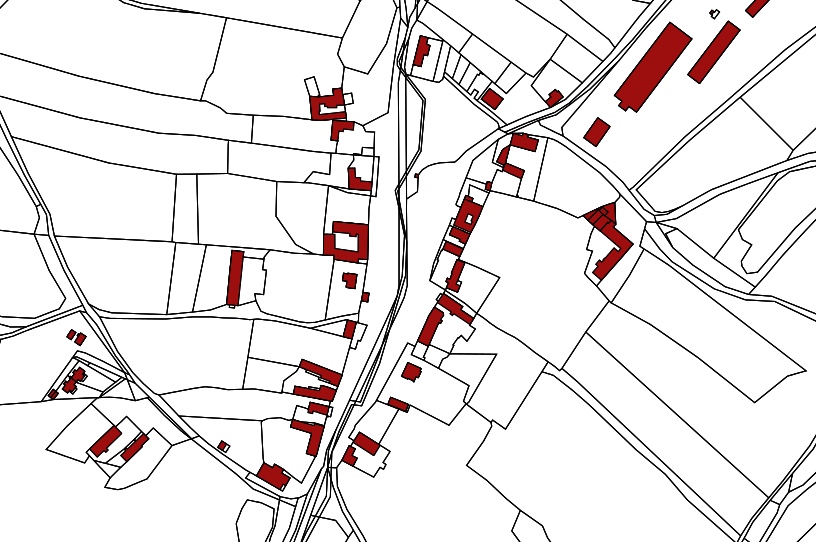
\includegraphics[width=.7\textwidth]{images/grass_ukazka.png}
\caption[Ukázka načtení VFK pomocí VFK Driveru GDAL v~programu GRASS GIS]{Ukázka načtení VFK pomocí VFK Driveru GDAL v~programu GRASS GIS (zdroj: vlastní)}
\end{figure}



\clearpage
\chapter{Použité technologie}

\section{QGIS}

QGIS je geografický informační systém, který je distribuován jako
open-source\footnote{Open-source software je takový software, k~němuž
  zákazník dostane od jeho tvůrce zdrojový kód a~může jej dále
  upravovat. Jednotlivé definice termínu \uv{open source} se liší
  zvláště v~podmínkách pro další distribuci
  softwaru.\cite{abclinuxu_opensource}} pod licencí \textit{GNU
  General Public License}. Je oficiálním a~klíčovým produktem
organizace OSGeo. Díky přenositelnosti zdrojového kódu je použitelný
na širokém spektru platforem, ať už jsou to desktopové platformy
Linux, MacOS, Windows, nebo mobilní platforma Android.

\begin{figure}[htb]
\centering

\includegraphics[scale=1]{images/qgis-logo.png}
\caption[QGIS -- logo]{QGIS -- logo (zdroj: \cite{qgis})}
\end{figure}

Program umožňuje prohlížení, tvorbu a~editaci velkého množství
vektorových (Esri Shapefile, GeoJSON, GPX, \dots), ale i~rastrových
(GeoTIFF, JPEG, \dots) nebo databázových (PostGIS) formátů. Podporuje zpracování
dat GPS a~tvorbu mapových výstupů. Mimo jiné umožňuje provádět
prostorové analýzy, analýzy terénu nebo analýzy síťové, práci
s~mapovou algebrou a~mnoho dalšího.

QGIS nedisponuje tak širokou paletou nástrojů, jako jeho open-source
kolega GRASS GIS. Jeho funkcionalita ale může být rozšířena díky
nepřebernému množství zásuvných modulů. Jedním z~nejdůležitějších
modulů pro analýzu geografických dat je zásuvný modul GRASS GIS, který
zpřístupňuje funkce stejnojmenného programu. QGIS poté může sloužit
jako jeho nadstavba.  \cite{qgis} \cite{qgis_wiki}


\section{GDAL}
\label{l_gdal}

GDAL je knihovna určená pro čtení a~zápis rastrových GIS
formátů. Knihovna je vyvíjena pod hlavičkou Open Source Geospatial
Foundation a~vydávána pod licencí \textit{X/MIT}. Knihovna používá
jednoduchý abstraktní datový model pro všechny podporované datové
formáty. Kromě toho nabízí také řadu užitečných nástrojů pro
příkazovou řádku určených pro konverzi a~zpracování
dat. \cite{gdal_wiki}

\begin{figure}[h]
\centering

\includegraphics[scale=1]{images/gdal-logo.png}
\caption[GDAL -- logo]{GDAL -- logo (zdroj: \cite{gdal})}
\end{figure}

GDAL byla původně vyvíjena Frankem Warmerdamem a~to do verze 1.3.2,
posléze byla knihovna převedena na GDAL Project Management Committee,
která je součástí Open Source Geospatial Foundation.\cite{gdal_wiki}

Knihovna OGR, která je od verze 2.0 součástí knihovny GDAL, slouží pro
práci s~daty ve vektorovém formátu.\cite{gdal}

GDAL je považován za jeden z~hlavních open-source projektů. Knihovna
je hojně využívána také v~komerční GIS sféře. Knihovna je otevřená
a~poskytuje základní funkcionalitu potřebnou pro denní práci
s~rozsáhlým množstvím GIS formátů.\cite{gdal_wiki}


\section{Python}

Jazyk Python je objektově orientovaný programovací jazyk, který
efektivně používá víceúrovňové datové typy. Jedná se o~jazyk
interpretovaný, čímž se jeví jako ideální nástroj pro psaní skriptů,
ale i~rychlý vývoj aplikací. Je vyvíjen jako open-source software,
díky čemuž se stává použitelným na velkém množství platforem (Linux,
Windows, MacOS, \dots). Jazyk je rozšířitelný o~široké spektrum
modulů, které umožňují řešit problematiku takřka z~jakékoli
oblasti. V~současné době je Python vyvíjen ve dvou verzích, ve verzi
2.x a~v~novější verzi 3.x.  \cite{dive_into_python} \cite{python_web}

\begin{figure}[htb]
\centering

\includegraphics[scale=.7]{images/python-logo.png}
\caption[Python -- logo]{Python -- logo (zdroj: \cite{python_web})}
\end{figure}

\newpage
\section{PyQt}

PyQt je modul, který zpřístupňuje knihovnu Qt pro programovací jazyk
Python. Spolu s~PySide se jedná o~nejznámější a~nejpoužívanější modul
pro Python postavený nad knihovnou Qt. Je vyvíjen britskou firmou
Riverbank Computing ve dvou verzích. Ve verzi 4, podporující knihovnu
Qt 4, a~ve verzi 5, která podporuje novější verzi Qt knihovny. Modul
je dostupný na všech platformách, které podporují knihovnu Qt
(Windows, MacOS/X a~Linux). PyQt je šířeno pod tzv. dvojí licencí,
\textit{GNU GPL v3} a~\textit{Riverbank Commercial License}. Spolu
s~těmito licencemi je dostupné i~pod komerční licencí.

\begin{figure}[htb]
\centering

\includegraphics[scale=1]{images/pyqt-logo.png}
\caption[PyQt -- logo]{PyQt -- logo (zdroj: \cite{pyqt_wiki})}
\end{figure}

Pro grafický návrh aplikace je vhodné použít nativní grafické
uživatelské rozhraní Qt Designer. Výstupem z~tohoto programu je soubor
obsahující vzhled aplikace ve formátu \textit{XML}. PyQt je poté
schopné tento formát převést do kódu jazyka Python. Pro komunikaci
mezi objekty je využíváno signálů a~slotů, díky čemuž je vytvoření
komponent velice snadné.

PyQt v~sobě kombinuje mocnost knihovny Qt s~jednoduchostí jazyka
Python, což z~něj dělá výkonný nástroj pro vývoj grafických aplikací.
\cite{pyqt} \cite{pyqt_wiki}


% =============================================================================
\clearpage
\chapter{Informační systém katastru nemovitostí}
\label{l_iskn}

ISKN je integrovaný informační systém pro podporu výkonu státní správy
katastru nemovitostí a~pro zajištění jeho uživatelských
služeb. Obsahuje prostředky pro současné vedení souborů popisných
informací (SPI) a~souborů geodetických informací (SGI). Dále jsou
v~něm obsaženy prostředky pro podporu správních a~administrativních
činností při vedení katastru nemovitostí a~pro správu dokumentačních
fondů. \cite{iskn}

\begin{figure}[htb]
\centering

\includegraphics[scale=1]{images/cuzk-logo.png}
\caption[ČUZK -- logo]{ČUZK -- logo (zdroj: \cite{iskn})}
\end{figure}

\section{Historie a~vývoj}

Vývoj systému byl započat v~roce 1997 ve spolupráci se společností APP
Czech s.r.o.\footnote{Dnes společnost funguje pod názvem NESS Czech
  s.r.o.}, která fungovala jako systémový integrátor a~dodavatel
aplikačního programového vybavení. Dalšími společnostmi podílejícími
se na vývoji ISKN byly Infinity, a.s., Compaq Computer
s.r.o.\footnote{Dnes pod názvem HP.}, Oracle Czech, s.r.o., Bentley
Systems, s.r.o., BEA Systems, s.r.o. \cite{iskn}

Systém byl nasazen do provozu v~září roku 2001, a~to na všech
katastrálních pracovištích včetně centrály. Dolaďování a~převzetí
závěrečných etap probíhalo v~roce 2002. V~témže roce byl dokončen
audit systému. \cite{iskn}

Implementace ISKN plně nahradila dřívější způsob vedení katastru
nemovitostí. ISKN integroval vedení a~správu katastru nemovitostí pod
jediný informační systém společný pro všechna pracoviště katastrálních
úřadů a~centrum. Toto vede k~tomu, že je možné zveřejňovat
a~poskytovat aktuální data z~katastru nemovitostí prostřednictvím
dálkového přístupu během několika málo minut, a~to z~celého území
republiky. \cite{iskn}

Data jsou do systému ISKN ukládána pomocí Spatial Cartridge Option do
databáze Oracle. Podpora vzdáleného přístupu k~datům pomocí sítě
Internet je zajištěna pomocí BEA WebLogic. Systémový management
využívá nástrojů CA Unicenter. \cite{iskn}

V~roce 2004 byla uzavřena nová smlouva se společností NESS Czech
s.r.o. na rozvoj a~údržbu informačního systému v~letech 2004 --
2006. V~tomto období byl zmodernizován především Dálkový přistup do
katastru nemovitostí a~zavedena orientační mapa parcel. Důležitou
inovací bylo zavedení elektronické značky pro výpis z~katastru
nemovitostí a~pro kopii katastrální mapy \footnote{Tento krok umožnil,
  aby tzv. \uv{ověřující} podle zákona č. 365/2000 Sb., o~informačních
  systémech veřejné správy, v~platném znění, mohli poskytovat ověřené
  výpisy z~katastru nemovitostí, převedené z~elektronické do listinné
  podoby. \cite{iskn}}. \cite{iskn}

Společnost NESS Czech s.r.o. poté v~dalších letech vyhrála několik
veřejných zakázek týkajících se údržby a~rozvoje ISKN. Hlavním cílem
bylo převedení decentralizovaného systému (107 lokálních databází
replikovaných do centrální databáze) na centralizovaný systém, ve
kterém byla data ISKN uložena pouze v~jedné databázi. Spolu s~touto
úpravou byla změněna i~architektura z~původní client/server na
třívrstvou architekturu. Architektura je postavena na platformě Oracle
Forms/Reports 10g a~databázi Oracle 10g. Další změnou byl přechod na
vyšší verzi Bentley nástroje pro správu prostorových dat. \cite{iskn}

ISKN byl nadále zlepšován. Za zmínku stojí především systém pro
Dálkový přístup do katastru nemovitostí nebo zavedení možnosti získat
informaci o~ukončení řízení pomocí SMS nebo e-mailové
zprávy. \cite{iskn}


\section{Hlavní charakteristiky ISKN}

\subsection{Optimalizace uložení dat}

Díky zvolení jednotného datového modelu pro uložení popisných
a~prostorových dat v~databázi Oracle spolu s~daty týkajících se
správních řízení byla umožněna současná aktualizace popisných
a~prostorových dat a~udržení jejich vzájemné konzistence. Pro
optimalizaci byla také přijata koncepce samostatné evidence budov
a~bezešvé digitální katastrální mapy. Od konce roku 2001 jsou
uchovávány také veškerá historická data popisných a~prostorových dat,
díky čemuž je možné sestavovat data do potřebných výstupů
k~historickému datu od zavedení ISKN v~roce 2001. \cite{iskn}

\subsection{Optimalizace procesů při správě KN}

Do systému ISKN byla zavedena celá řada automatických kontrol pro
proces zapsání změny do KN. Dále bylo umožněno převzetí aktuálních dat
z~jiných registrů (např. registr obyvatel) a~ostatních informačních
systémů. Postup provedení změny dat KN je následující: na základě
návrhu je připraven budoucí stav, který je možné před jeho zplatněním
zobrazit (SPI, SGI), případně v~něm provádět úpravy. Toto zajišťuje
důkladnou kontrolu výsledného stavu katastru. Proces realizace změny
je navíc zajištěn i~technicko-organizačními opatřeními (návrh změny
a~kontrolu, včetně zplatnění provádí vždy jiná osoba dle přidělených
uživatelských rolí). \cite{iskn}

Díky novým procesům ve zpracování dat/návrhů změn je možné částečné
nabytí platnosti geometrického plánu s~automatizovanou změnou návrhu
změny v~budoucím stavu. Nové procesy také umožňují aktualizaci dat
katastru nemovitostí takovým způsobem, aniž by zamkly aktualizovaná
data. Pouze se jimi řeší konflikty v~aktualizaci stejných dat.

Součástí ISKN je také jednotná centrální správa číselníků, která vnáší
jednotnost do procesu zpracování změn na katastrálních úřadech. Tímto
se rapidně zvyšuje konzistence a~kvalita datové základny. Některé
z~centrálních číselníků nebo seznamů jsou přebírány z~externích
datových zdrojů (např. číselníky územní identifikace,
PSČ). \cite{iskn}

\subsection{Bezpečnost}

Vysoká bezpečnost ochrany dat je zajištěna kombinací hardwarových
prostředků s~operačním systémem, databází a~vlastní aplikací
ISKN. Nepřetržitý provoz je zajištěn pomocí technologie databázových
a~aplikačních clusterů a~tím, že je celá infrastruktura zdvojena
(primární a~záložní centrum). Do záložního centra jsou replikována
veškerá data tak, aby byl v~případě náhlého výpadku primárního centra
zajištěn nepřetržitý provoz ISKN. \cite{iskn}


\section{Poskytování dat}

Poskytování dat je umožněno na základě vyhlášky číslo 358/2013 Sb.,
o~poskytování údajů z~katastru nemovitostí. \cite{iskn}

\subsection{Poskytování dat dálkovým přístupem}

Na základě registrace je umožněno poskytování dat (zdarma, nebo za
úplatu podle typu zákazníka) prostřednictvím sítě Internet. Výpisy
z~KN a~snímky katastrální mapy mají povahu veřejných elektronických
listin (jsou opatřeny elektronickou značkou) a~mohou být převedeny do
podoby listinných veřejných listin. Tímto způsobem je v~současné době
vyřizována více než třetina výstupů. \cite{iskn}

Více informací o~této metodě poskytování dat je spolu s~aplikací
dostupných na stránkách ČUZK (\url{http://www.cuzk.cz/aplikace-dp/}).

\subsection{Poskytování dat ve výměnném formátu ISKN}

Data z~KN mohou být poskytována v~textovém souboru, který obsahuje
záznamy v~pevně definované struktuře. Více informací o~tomto výměnném
formátu je uvedeno v~kapitole č. \ref{l_format_vfk}.


% ==================================================================================
\clearpage
\chapter{Výměnný formát ISKN}
\label{l_format_vfk}

V~této kapitole je ve stručnosti popsána historie vývoje výměnného
formátu ISKN spolu s~jeho popisem, ve kterém se věnuji především
sekcím důležitým pro vývoj zásuvného modulu pro QGIS, který dokáže
data v~tomto formátu zobrazit.

\section{Vývoj formátu}

Hlavním milníkem ve vývoji výměnného formátu bylo zavedení ISKN,
viz. kapitola č. \ref{l_iskn}. Do této doby byly soubory SPI a~SGI
ukládány odděleně, což se právě se zavedením ISKN změnilo. Tento krok
vedl k~vytvoření nového výměnného formátu (NVF), který postupně
nahrazoval starý výměnný formát (SVF). \cite{dp_landa}

\subsection{Výměnný formát KN před ISKN}

Tento formát je po zavedení nového formátu také nazýván \textit{starý
  výměnný formát}~--~\textbf{SVF}. Byl vytvořen roku 1996, kdy začala
vznikat digitalizace SGI. Obsahuje dvě samostatné části:

\begin{enumerate}
 \item \textbf{SPI} -- Obsahuje informace o~vlastnících, parcelách a~nabývacích titulech. Byl distribuován ve dvou formátech:
 \begin{enumerate}
  \item soubory ve formátu \textit{.dbf}: Tento typ souboru byl dále dělen na další dvě části:
  
  \begin{enumerate}
   \item SPI bez jiných právních vztahů (bez JPV),
   \item SPI s~jinými právními vztahy (s~JPV).
  \end{enumerate}
  
  \item soubory ve formátu \textit{.txt}: SB, SC, SE
 \end{enumerate}
 
 Data byla poskytována v~následujících rozsazích: podle územní
 jednotky (katastrální území, obec, okres, ČR), dle výběru parcel,
 nebo na základě oprávněného subjektu (pouze ve formátu
 \textit{.txt}).
 
 Ve výše zmíněných formátech (\textit{.dbf, .txt}) jsou značné
 nesoulady. Ty jsou způsobeny hlavně neexistencí některých položek
 v~novém datovém modelu ISKN nebo jejich rozdílnou interpretací.

 \item \textbf{SGI} -- Jsou v~něm obsaženy informace o~poloze nemovitostí. 
 
   Data byla poskytována pro katastrální území, kde již byla provedena
   digitalizace.
\end{enumerate}

V~současné době je již oficiální podpora ukončena a~byl nahrazen právě
novým výměnným formátem. \cite{svf_cuzk}

\subsection{Výměnný formát VF ISKN}

Formát je nazýván také jako \textit{nový výměnný formát} --
\textbf{NVF}. V~tomto formátu jsou obsaženy zároveň popisné i~grafické
informace včetně dat o~řízení. Data jsou vytvářena ve dvou stavech:

\begin{itemize}
\item \textbf{Stavová data} -- Data jsou vygenerována vzhledem ke
  konkrétnímu časovému okamžiku. Obsahují vždy kompletní data pro daný
  okamžik. Práce s~těmito daty je řešena v~původní verzi zásuvného
  modulu pro QGIS.
 
\item \textbf{Změnová data} -- Jsou v~nich obsaženy pouze změny za
  požadovaný časový úsek. Zpracováním a~zobrazením změnových dat
  v~programu QGIS se zabývá právě tato diplomová práce.
\end{itemize}

Data jsou poskytována v~následujících rozsazích:

\begin{itemize}
 \item územní jednotka (katastrální území, obec, okres, ČR),
 \item oprávněný subjekt,
 \item výběr parcel,
 \item výběr parcel polygonem v~mapě.
\end{itemize}

Do výměnného souboru je možné dle přání zákazníka vybrat libovolné
kombinace datových skupin, viz
tab. \ref{t_datove_skupiny}. \cite{dp_landa}

\begin{table}[htbp]
\centering
\caption[Datové skupiny VF ISKN]{Datové skupiny VF ISKN (zdroj: \cite{nvf_cuzk})}
\begin{tabular}{ll}
\toprule
\textbf{Název skupiny} & \textbf{Obsah} \\ 
\midrule
Nemovitosti & parcely a~budovy \\ 
Jednotky & bytové jednotky \\ 
Bonitní díly parcel & kódy BPEJ k~parcelám \\ 
Vlastnictví & \parbox{220pt}{listy vlastnictví, oprávněné subjekty a~vlastnické vztahy} \\ 
Jiné právní vztahy & ostatní právní vztahy kromě vlastnictví \\ 
Řízení & údaje o~řízení (vklad, záznam,…) a~listiny \\ 
Prvky katastrální mapy & katastrální mapy v~digitální podobě \\ 
BPEJ & hranice BPEJ včetně kódů \\ 
Geometrický plán & geometrické plány \\ 
Rezervovaná čísla & rezervovaná parcelní čísla a~čísla PBPP \\ 
Definiční body & definiční body parcel a~staveb \\ 
Adresní místa & adresní místa budov \\
\bottomrule
\end{tabular}
\label{t_datove_skupiny}
\end{table}

\newpage
\section{Struktura výměnného formátu ISKN}

Tato kapitola pojednává o~struktuře výměnného formátu ISKN. Nejsou zde
popsány a~do detailu rozvedeny veškeré datové bloky formátu, ale pouze
ty nejdůležitější prvky formátu vzhledem k~zásuvnému modulu pro
QGIS. Podrobný popis formátu je dostupný v~oficiální dokumentaci
(\cite{vfk_struktura}), ze které tato kapitola čerpá. Veškeré ukázky
výměnného formátu jsou pořízeny z~testovacích dat dostupných na
stránkách ČUZK (\cite{nvf_cuzk}).

Datový soubor \textit{.vfk} se skládá ze tří základních částí, které
budou samostatně popsány na následujících řádcích této kapitoly:

\begin{itemize}
 \item hlavička \texttt{\&H},
 \item datové bloky \texttt{\&B},
 \item koncový znak \texttt{\&K}.
\end{itemize}

Datový soubor je vytvářen v~kódování češtiny dle ČSN ISO 8859-2 (ISO
Latin2)\footnote{Ve výjimečných případech je možné použít kódování
  WIN1250. Toto kódování je použito i~v~souboru ve formátu XML verze
  1.0.}. Desetinným oddělovačem je tečka (.). Datum a~čas je uveden ve
tvaru ``03.06.1999 09:58:42''. Jednotlivé záznamy na řádcích jsou
odděleny pomocí středníku (;). Každá datová věta je ukončena pomocí
souslednosti znaků \texttt{<CR><LF>}. Znak \uv{\texttt{\currency}}
znamená, že následující řádek souboru výměnného formátu je
pokračováním předchozího řádku a~tvoří jedinou datovou větu, která
v~textové položce obsahuje formátovací znaky
\texttt{<CR><LF>}. \cite{vfk_struktura}

\subsection{Hlavička \texttt{\&H}}

Každý řádek hlavičky začíná sousledností znaků \texttt{\&H}, po které
následuje označení položky, např. \texttt{VERZE}. Jednotlivé údaje
jsou odděleny pomocí středníku. Hlavička obsahuje několik povinných
řádků, jejichž seznam je uveden v~tabulce \ref{t_hlavicka}.

\begin{table}[htbp]
\centering
\caption[Seznam položek hlavičky]{Seznam položek hlavičky (zdroj: \cite{vfk_struktura})}
\begin{tabular}{ll}
\toprule
\textbf{Položka} & \textbf{Popis} \\ 
\midrule
VERZE & označení verze VF \\ 
VYTVORENO & datum a~čas vytvoření souboru \\ 
PUVOD & původ dat \\ 
CODEPAGE & označení kódové stránky \\ 
SKUPINA & seznam skupin datových bloků souboru \\ 
JMENO & jméno osoby, která soubor vytvořila \\ 
PLATNOST & časová podmínka použitá pro vytvoření souboru \\ 
ZMENY & stavová, nebo změnová data \\ 
POLYG & omezující podmínka -- polygon \\
KATUZE & omezující podmínka -- katastrální území \\
OPSUB & omezující podmínka -- oprávněné subjekty \\
PAR & omezující podmínka -- parcely \\
\bottomrule
\end{tabular}
\label{t_hlavicka}
\end{table}

Příklad prvních řádků hlavičky je uveden v~tabulce
\ref{t_hlavicka_priklad}. Tabulka byla vytvořena na základě
testovacích dat a~obsahuje i~některé nepovinné položky,
např. \texttt{\&HINFO}.

\begin{table}[htbp]
\centering
\caption[Ukázka hlavičky]{Ukázka hlavičky (zdroj: \cite{vfk_struktura})}
\begin{tabular}{ll}
\toprule
\textbf{Položka} & \textbf{Atributy} \\ 
\midrule
\&HVERZE & "5.0" \\ 
\&HINFO & "TESTOVACÍ" \\ 
\&HVYTVORENO & "23.11.2013 12:58:06" \\ 
\&HPUVOD & "ISKN" \\ 
\&HCODEPAGE & "WE8ISO8859P2" \\ 
\&HSKUPINA & "NEMO";"JEDN";"BDPA";"VLST";"JPVZ" \\ 
\&HJMENO & "Kokeš Petr Ing." \\ 
\&HPLATNOST & "23.11.2013 12:51:00";"23.11.2013 12:51:00" \\ 
\&HZMENY & 0 \\ 
\&HNAVRHY & 0 \\ 
\&HPOLYG & 0 \\ 
\bottomrule
\end{tabular}
\label{t_hlavicka_priklad}
\end{table}

\begin{description}
 \item[VERZE:] Pouze jeden řádek označující verzi souboru VFK.
 \item[VYTVOŘENO:] Datum a~čas, kdy byl datový soubor vygenerován.
 \item[PŮVOD:] Specifikuje původ dat. Standardně je zde uvedeno
   \uv{ISKN}.
 \item[CODEPAGE:] Označení kódové stránky. Hodnota \uv{WE8ISO8859P2}
   značí kódování češtiny dle ČSN ISO 8859-2. Hodnota
   \uv{"EE8MSWIN1250} slouží pro označení kódování češtiny dle MS
   WIN1250.
 \item[SKUPINA:] Uvádí se zde seznam datových bloků
   souboru. Např. \texttt{\&HSKUPINA; ”Zkratka skupiny“;[“Zkratka
     skupiny” \dots]}.
 \item[JMÉNO:] Jméno osoby, která soubor
   vytvořila. Např. \texttt{\&HJMENO;"Jméno Příjmení"}.
 \item[PLATNOST:] Časová podmínka použitá pro vytvoření souboru. Zde
   jsou možné dvě varianty:
 
 \begin{itemize}
 \item Data jsou platná v~daném čase. \texttt{\&HPLATNOST;"03.12.2013
     09:56:42"; "03.12.2013 09:56:42"},
 \item data jsou platná v~daném
   období. \texttt{\&HPLATNOST;"03.12.2012 09:56:42"; "03.12.2013
     09:56:42"}.
 \end{itemize}
 
 S~tímto souvisí položka \texttt{\&HZMENY}, která nabývá hodnot 0/1
 a~označuje, zda se jedná o~data stavová, nebo změnová. Položka
 \texttt{\&HNAVRHY} nabývá také hodnot 0/1 a~značí, zda jsou v~souboru
 obsaženy potvrzené geometrické plány, či nikoliv.
 
\item[KATUZE:] Obsahuje jeden řádek, který popisuje hlavičku omezující
  podmínky katastrálních území. Další řádky začínající \texttt{\&D}
  tvoří omezující podmínku. Počet datových řádků udává počet
  katastrálních území, která omezující podmínku tvoří. Pokud
  v~omezující podmínce není žádné katastrální území, bude uvedena
  pouze hlavička. Pro ujasnění je zde uveden příklad z~testovacích
  dat.
 
 \begin{lstlisting}
&HKATUZE;KOD N6;OBCE_KOD N6;NAZEV T48;PLATNOST_OD D;PLATNOST_DO
&DKATUZE;693936;550426;"Jama";"19.06.1991 00:00:00";""
 \end{lstlisting}

\item[OPSUB:] První řádek popisuje hlavičku omezující podmínky
  oprávněných subjektů. Další řádky s~daty poté omezující podmínku
  tvoří, obdobně jako je uvedeno u~omezující podmínky pro katastrální
  území. Počet datových řádků je shodný s~počtem oprávněných subjektů
  v~omezující podmínce.
 
\item[PAR:] První řádek popisuje hlavičku omezující podmínky
  parcel. Další řádky tvoří omezující podmínku. Počet datových řádků
  je shodný s~počtem parcel uvedených v~omezující podmínce.
 
\item[POLYG:] Tento údaj může nabývat hodnot 0/1. Pokud je uvedena
  hodnota 1, tak je obsah souboru odvozen z~polygonu. V~takovém to
  případě musí být polygon na dalších řádcích definován svými
  vrcholy. Takto zadaný polygon může mít nejvýše 101 vrcholů. Příklad
  zadání omezujícího polygonu:
 
 \begin{lstlisting}
&HPOLYGDATA;675124.12;1024587.24
&HPOLYGDATA;675224.12;1024687.24
&HPOLYGDATA;675184.12;1024537.24
 \end{lstlisting} 
\end{description}

\subsection{Datové bloky}

Datové bloky obsahují řádky dvojího typu:

\begin{itemize}
\item uvozující řádek bloku \texttt{\&B} -- obsahuje seznam atributů
  s~jejich datovými typy, viz tab. \ref{t_datove_typy},
 \item datové řádky \texttt{\&D} -- v~řádku jsou uvedeny vlastní data.
\end{itemize}

\begin{table}[htbp]
\centering
\caption[Datové typy ISKN]{Datové typy ISKN (zdroj: \cite{dp_landa})}
\begin{tabular}{lll}
\toprule
\textbf{Kód} & \textbf{Datový typ} & \textbf{Číslo za kódem} \\ 
\midrule
N & číselný & maximální délka položky \\ 
T & textový & maximální délka textu \\ 
D & datumový & ve tvaru DD.MM.YYYY HH:MI:SS \\ 
\bottomrule
\end{tabular}
\label{t_datove_typy}
\end{table}

Níže je uveden příklad datového bloku pro blok \uv{PARCELA}. Ukázka je
pořízena z~testovacích dat.

\begin{lstlisting}
  &BPAR;ID N30;STAV_DAT N2;DATUM_VZNIKU D;DATUM_ZANIKU
  D;PRIZNAK_KONTEXTU N1;RIZENI_ID_VZNIKU N30;RIZENI_ID_ZANIKU
  N30;PKN_ID N30;PAR_TYPE T10;KATUZE_KOD N6;KATUZE_KOD_PUV
  N6;DRUH_CISLOVANI_PAR N1;KMENOVE_CISLO_PAR N5;ZDPAZE_KOD
  N1;PODDELENI_CISLA_PAR N3;DIL_PARCELY N1;MAPLIS_KOD N30;ZPURVY_KOD
  N1;DRUPOZ_KOD N2;ZPVYPA_KOD N4;TYP_PARCELYN1;VYMERA_PARCELY
  N9;CENA_NEMOVITOSTI N14.2;DEFINICNI_BOD_PAR T100;TEL_ID N30;PAR_ID
  N30;BUD_ID N30;IDENT_BUD T1;SOUCASTI T1;PS_ID N30;IDENT_PS T1

  &DPAR;3067989306;0;"26.06.2003 07:43:05";"";3;3003873306;;;"PKN";
  693936;;1;37;;1;;6780;2;13;;;332;;"";674674306;;323700306;"a";"n";;"n"
\end{lstlisting}

\subsection*{Seznam skupin datových bloků ISKN}

V~této sekci je uveden popis jednotlivých skupin datových bloků. Jsou
zde uvedeny pouze nejpodstatnější informace, podrobný popis lze
dohledat v~oficiální dokumentaci formátu VFK (\cite{vfk_struktura}).

\begin{description}
\item[NEMOVITOSTI:] Jedná se o~největší skupinu datových bloků. Celkem
  jich může obsahovat až 21. V~této skupině se nachází dva
  nejdůležitější bloky z~pohledu zásuvného modulu pro QGIS, a~to bloky
  PAR a~BUD. Právě tyto dva bloky jsou pomocí zásuvného modulu
  vizualizovány. Dále je zde obsažen například číselník způsobů
  využití pozemku nebo způsob využití budov. Seznam všech bloků v~této
  skupině je uveden v~tabulce \ref{t_skupina_nemovitosti}. Znak (*)
  uvedený v~tabulce znamená, že daný blok nepodléhá historizaci.
 
\begin{table}[htbp]
\centering
\caption[Seznam datových bloků ve skupině \uv{NEMOVITOSTI}]{Seznam datových bloků ve skupině \uv{NEMOVITOSTI} (zdroj: \cite{vfk_struktura})}
\begin{tabular}{ll}
\toprule
\textbf{Kód} & \textbf{Popis} \\ 
\midrule
PAR & Parcely \\ 
BUD & Budovy \\ 
CABU & Části budov \\ 
ZPOCHN* & Číselník způsobů ochrany nemovitosti \\
DRUPOZ* & Číselník druhů pozemku \\
ZPVYPO* & Číselník způsobů využití pozemku \\
ZDPAZE* & Číselník zdrojů parcel ZE \\
ZPURVY* & Číselník způsobů určení výměry \\
TYPBUD* & Číselník typů budov \\
MAPLIS* & Číselník mapových listů \\
KATUZE* & Číselník katastrálních území \\
OBCE* & Číselník obcí -- vázaně \\
CASOBC* & Číselník částí obce -- vázaně \\
OKRESY* & Číselník okresů -- vázaně \\
KRAJE* & Číselník krajů -- vázaně \\
NKRAJE* & Číselník nových krajů -- vázaně \\
RZO & Přiřazení způsobu ochrany k~nemovitostem \\
ZPVYBU* & Způsob využití budov \\
PS & Práva stavby \\
RU & Přiřazení účelu práva stavby \\
UCEL & Číselník účelů práva stavby \\
\bottomrule
\end{tabular}
\label{t_skupina_nemovitosti}
\end{table}
 
\item[JEDNOTKY:] V~této skupině jsou uvedeny bytové či nebytové
  prostory, které byly označeny příslušnou listinou jako jednotka. Pro
  každou jednotku je uveden její popis (jednoznačně ji identifikuje
  v~rámci budovy), typ a~způsob využití. Ke každé jednotce je dále
  uveden spoluvlastnický podíl
  ($\frac{\text{velikost podlahové plochy}}{\text{celková plocha všech
      jednotek v~domě}}$). \cite{dp_landa}
 
 
\begin{table}[htbp]
\centering
\caption[Seznam datových bloků ve skupině \uv{JEDNOTKY}]{Seznam datových bloků ve skupině \uv{JEDNOTKY} (zdroj: \cite{vfk_struktura})}
\begin{tabular}{ll}
\toprule
\textbf{Kód} & \textbf{Popis} \\ 
\midrule
JED & Jednotky \\ 
TYPJED* & Číselník typů jednotek \\ 
ZPVYJE* & Způsob využití jednotek \\ 
\bottomrule
\end{tabular}
\label{t_skupina_jednotky}
\end{table}

 \newpage
\item[BONITNÍ DÍLY PARCEL:] Jsou zde uvedeny informace o~bonitních
  dílech parcely. Ve skupině se nachází pouze jeden datový blok (BDP),
  ve kterém je popsán vztah mezi BPEJ\footnote{\textbf{Bonitovaná
      půdně-ekologická jednotka}: Základní určovací a~oceňovací
    jednotka produkční schopnosti zemědělské půdy. Je vyjádřená
    číselným kódem -- číslice kódu vyjadřují půdně-klimatické
    vlastnosti půdy. Jednotky tvoří ohraničený územní celek, který má
    specifické ekologické vlastnosti a~bioenergetický
    potenciál. \cite{vugtk}} a~parcelou. \cite{dp_landa}
 
\item[VLASTNICTVÍ:] Tato skupina bloků obsahuje informace
  o~vlastnictví. Jako vlastník zde může být uvedena fyzická osoba,
  právnická osoba nebo jiný oprávněný uživatel (manželé v~bezpodílovém
  spoluvlastnictví). Ve skupině se může nacházet několik datových
  bloků, viz tab. \ref{t_skupina_vlastnictvi}. \cite{dp_landa}
 
\begin{table}[htbp]
\centering
\caption[Seznam datových bloků ve skupině \uv{VLASTNICTVÍ}]{Seznam datových bloků ve skupině \uv{VLASTNICTVÍ} (zdroj: \cite{vfk_struktura})}
\begin{tabular}{ll}
\toprule
\textbf{Kód} & \textbf{Popis} \\ 
\midrule
OPSUB & Oprávněné subjekty \\ 
VLA & Vlastnictví \\ 
CHAROS* & Číselník charakteristik oprávněných subjektů \\ 
TEL & Katastrální tělesa \\
\bottomrule
\end{tabular}
\label{t_skupina_vlastnictvi}
\end{table}

\item[JINÉ PRÁVNÍ VZTAHY:] Obsahuje informace o~jiných než
  vlastnických vztazích jednoho oprávněného subjektu (nemovitosti) ke
  konkrétnímu předmětu (nemovitosti, vlastnictví, dalšímu jinému
  právnímu vztahu). Seznam a~popis datových bloků je uveden v~tabulce
  č. \ref{t_skupina_jpv}. \cite{dp_landa}
 
\begin{table}[htbp]
\centering
\caption[Seznam datových bloků ve skupině \uv{JINÉ PRÁVNÍ VZTAHY}]{Seznam datových bloků ve skupině \uv{JINÉ PRÁVNÍ VZTAHY} (zdroj: \cite{vfk_struktura})}
\begin{tabular}{ll}
\toprule
\textbf{Kód} & \textbf{Popis} \\ 
\midrule
JPV & Jiné právní vztahy \\ 
TYPRAV* & Číselník typů právních vztahů \\ 
RJPV & Vazba JPV k~jinému věcnému právu \\ 
\bottomrule
\end{tabular}
\label{t_skupina_jpv}
\end{table}

\item[ŘÍZENÍ:] Tato skupina je druhou nejobsáhlejší skupinou ve
  výměnném formátu. Může být obsažena ve změnovém exportu z~ISKN --
  v~tomto případě obsahuje pouze záznamy, které byly v~daném časovém
  intervalu změněny. Obsahuje několik datových bloků, viz
  tab. \ref{t_skupina_rizeni}. \cite{dp_landa}
 
\begin{table}[htbp]
\centering
\caption[Seznam datových bloků ve skupině \uv{ŘÍZENÍ}]{Seznam datových bloků ve skupině \uv{ŘÍZENÍ} (zdroj: \cite{vfk_struktura})}
\begin{tabular}{ll}
\toprule
\textbf{Kód} & \textbf{Popis} \\ 
\midrule
RIZENI* & Řízení (vklad, záznam) \\ 
RIZKU* & Vazba Řízení -- Katastrální území \\ 
OBJRIZ* & Objekty řízení (parcely, budovy, \dots) \\ 
PRERIZ* & Předměty řízení \\ 
UCAST* & Účastníci řízení \\ 
ADRUC* & Adresy účastníků řízení \\ 
LISTIN* & Listiny \\ 
DUL* & Další údaje listin \\ 
LDU* & Vazba Listiny -- Další údaje listin \\ 
TYPLIS* & Číselník typů listin \\ 
TYPPRE* & Číselník typů předmětu řízení \\ 
TYPRIZ* & Typy řízení \\ 
TYPUCA* & Typy účastníků řízení \\ 
UCTYP* & Vazba Účastnící -- Typy účastníků řízení \\ 
RL & Přiřazení listin k~nemovitostem, vlastnictví a~jiným právním vztahům \\ 
OBESMF* & Obeslání účastníků řízení \\ 
\bottomrule
\end{tabular}
\label{t_skupina_rizeni}
\end{table}
 
\item[PRVKY KATASTRÁLNÍ MAPY:] Tato skupina je jednou
  z~nejdůležitějších pro zásuvný modul, respektive pro driver VFK
  v~knihovně GDAL. Jsou v~ní totiž obsaženy jak popisné, tak hlavně
  polohopisné informace o~prvcích polohopisu. Z~nich (tedy hlavně
  z~prvních dvou datových bloků \texttt{SOBR} a~\texttt{SBP}) je
  tvořena geometrie vektorové mapy. Spolu s~nimi skupina obsahuje
  další neméně důležité datové bloky, viz
  tab. \ref{t_skupina_prvkyKM}. \cite{dp_landa}

\begin{table}[htbp]
\centering
\caption[Seznam datových bloků ve skupině \uv{PRVKY KATASTRÁLNÍ MAPY}]{Seznam datových bloků ve skupině \uv{PRVKY KATASTRÁLNÍ MAPY} (zdroj: \cite{vfk_struktura})}
\begin{tabular}{ll}
\toprule
\textbf{Kód} & \textbf{Popis} \\ 
\midrule
SOBR* & Souřadnice obrazu bodů polohopisu v~mapě \\ 
SBP & Spojení bodů polohopisu -- definuje polohopisné liniové prvky \\ 
SBM & Spojení bodů mapy -- definuje nepolohopisné liniové prvky \\ 
KODCHB* & Číselník kódů charakteristiky kvality bodu \\ 
TYPSOS* & Číselník typů souřadnicových systémů \\ 
HP & Hranice parcel \\ 
OP & Obrazy parcel (parcelní číslo, značka druhu pozemku, \dots) \\ 
OB & Obrazy budov (obvod budovy, značka druhu budovy) \\ 
DPM & Další prvky mapy \\ 
OBBP & Obrazy bodů BP \\ 
TYPPPD* & Číselník typů prvků prostorových dat \\ 
ZVB & Zobrazení věcných břemen \\ 
POM & Prvky orientační mapy \\ 
SPOM & Spojení prvků orientační mapy -- definuje liniové prvky \\ 
SPOL & Souřadnice polohy bodů polohopisu (měřené) \\  
\bottomrule
\end{tabular}
\label{t_skupina_prvkyKM}
\end{table}
 
 \newpage
\item[BPEJ:] Skupina \texttt{BPEJ} obsahuje dva datové bloky, viz
  tab. \ref{t_skupina_bpej}. Jsou v~ní obsaženy informace
  o~bonitovaných půdně ekologických jednotkách. BPEJ je základní
  mapovací a~oceňovací jednotka zemědělských půd, která vyjadřuje
  rozdílné produkční a~ekonomické efekty zemědělského území. Hranice
  BPEJ nejsou součástí katastrální mapy. Pouze tvoří rozhraní mezi
  dvěma jednotkami. \cite{dp_landa}

\begin{table}[htbp]
\centering
\caption[Seznam datových bloků ve skupině \uv{BPEJ}]{Seznam datových bloků ve skupině \uv{BPEJ} (zdroj: \cite{vfk_struktura})}
\begin{tabular}{ll}
\toprule
\textbf{Kód} & \textbf{Popis} \\ 
\midrule
HBPEJ & Hranice BPEJ \\ 
OBPEJ & Označení BPEJ \\ 
\bottomrule
\end{tabular}
\label{t_skupina_bpej}
\end{table}
 
\item[GEOMETRICKÝ PLÁN:] Tato skupina obsahuje sadu bloků popisujících
  geometrický plán a~hlavičku dalších změn v~KM, které nejsou
  prováděny geometrickým plánem. Obsahuje několik datových bloků,
  jejichž seznam je uveden v~tabulce č. \ref{t_skupina_gp}. Ve skupině
  je obsažena tabulka pro uchování záznamů podrobného měření změn jak
  v~terénu, tak i~změn, které s~měřením v~terénu nesouvisí (slučování
  parcel, demolice budov, \dots). \cite{dp_landa} \cite{vfk_struktura}

\begin{table}[htbp]
\centering
\caption[Seznam datových bloků ve skupině \uv{GEOMETRICKÝ PLÁN}]{Seznam datových bloků ve skupině \uv{GEOMETRICKÝ PLÁN} (zdroj: \cite{vfk_struktura})}
\begin{tabular}{ll}
\toprule
\textbf{Kód} & \textbf{Popis} \\ 
\midrule
NZ & Hlavičky geometrických plánů a~ostatních změn KM \\ 
ZPMZ & Hlavičky ZPMZ \\ 
NZZP & Vazební tabulka návrhy změn KM -- ZPMZ \\ 
PARG & Parcely GP \\ 
BUDG & Budovy GP \\ 
BDPG & Bonitní díly parcel GP \\ 
HPG & Hranice parcel GP \\ 
OPG & Obrazy parcel GP \\ 
OBG & Obrazy budov GP \\ 
ZVBG & Zobrazení věcných břemen GP \\ 
DPMG & Další prvky mapy GP \\ 
SBPG & Spojení bodu polohopisu GP \\ 
OBPEJG & Označení BPEJ GP \\ 
SBMG & Spojení bodů mapy GP \\ 
HBPEJG & Hranice BPEJ GP \\ 
OBDEBOG & Obrazy definičních bodů parcel a~budov GP \\ 
\bottomrule
\end{tabular}
\label{t_skupina_gp}
\end{table}

 \newpage
\item[REZERVOVANÁ ČÍSLA:] Rezervovanými čísly se v~této skupině myslí
  parcelní čísla, která byla rezervována pro účely vyhotovení
  geometrického plánu. Před potvrzením geometrického plánu probíhá
  kontrola, jestli byla použita přidělená rezervovaná parcelní
  čísla. Při zápisu nové parcely do KN se její číslo z~tabulky
  \texttt{RECI} maže. Úplné parcelní číslo musí být jedinečné v~rámci
  tabulek \texttt{PAR} a~\texttt{RECI}.
 
  Datový blok \texttt{DOCI} obsahuje všechna parcelní čísla, která kdy
  byla použita za dobu elektronického vedení katastru nemovitostí
  v~informačním systému ISKN (od r. 2001). Seznam všech datových bloků
  je uveden v~tabulce č. \ref{t_skupina_rezCisla}. \cite{dp_landa}
  \cite{vfk_struktura}

\begin{table}[htbp]
\centering
\caption[Seznam datových bloků ve skupině \uv{REZERVOVANÁ ČÍSLA}]{Seznam datových bloků ve skupině \uv{REZERVOVANÁ ČÍSLA} (zdroj: \cite{vfk_struktura})}
\begin{tabular}{ll}
\toprule
\textbf{Kód} & \textbf{Popis} \\ 
\midrule
RECI & Rezervovaná parcelní čísla \\
DOCI & Dotčená parcelní čísla \\
DOHICI & Dotčená historická parcelní čísla \\
REZBP & Rezervovaná čísla bodu PBPP \\
\bottomrule
\end{tabular}
\label{t_skupina_rezCisla}
\end{table}

\item[DEFINIČNÍ BODY:] Skupina obsahuje pouze jeden datový blok
  \texttt{OBDEBO}. V~tomto bloku jsou obsaženy obrazy definičních bodů
  parcel, budov a~částí budov (pokud jsou v~ISKN naplněny). Jsou zde
  uvedeny údaje o~souřadnicích a~odkazech (ID) na objekty
  v~KN. \cite{vfk_struktura}
 
\item[ADRESNÍ MÍSTA:] Datový blok \texttt{BUDOBJ} zajišťuje vazbu mezi
  budovami a~adresami pomocí ID budovy a~kódu objektu. Tento blok
  nepracuje s~historií -- obsahuje vždy aktuální data bez ohledu na
  datum, ke kterému je export NVF vytvořen.
 
  Ve druhém bloku (\texttt{ADROBJ}) jsou uvedeny odkazy na adresy
  budov, které jsou obsaženy v~bloku nemovitostí. Blok opět nepracuje
  s~historií. \cite{vfk_struktura}

\begin{table}[htbp]
\centering
\caption[Seznam datových bloků ve skupině \uv{ADRESNÍ MÍSTA}]{Seznam datových bloků ve skupině \uv{ADRESNÍ MÍSTA} (zdroj: \cite{vfk_struktura})}
\begin{tabular}{ll}
\toprule
\textbf{Kód} & \textbf{Popis} \\ 
\midrule
BUDOBJ & Odkazy objektů na adresy \\
ADROBJ & Adresy \\
\bottomrule
\end{tabular}
\label{t_skupina_adrMista}
\end{table}
 
\end{description}


\subsection{Koncový znak \texttt{\&K}}

Specifickou částí výměnného formátu je takzvaný \uv{koncový znak}
\texttt{\&K}. Načtení tohoto znaku signalizuje konec souboru výměnného
formátu. Pro driver VFK v~knihovně GDAL znak znamená konec načítání.


\section{Změnové věty v~NVF}
\label{l_struktura_zmen}
Změnový export nelze provést nad všemi skupinami datových bloků. Proveden může být pouze nad následujícími:

\begin{itemize}
\itemsep 1pt	
\parskip 1pt
 \item nemovitosti,
 \item jednotky,
 \item bonitní díly parcel,
 \item vlastnictví,
 \item JPV,
 \item řízení,
 \item prvky katastrální mapy,
 \item BPEJ.
\end{itemize}

Objekty, které byly vybrány v~parametrech při spuštění exportu, jsou
součástí datového souboru i~v~případě, kdy na nich nebyla provedena
žádná změna (tzn. jsou platné). Pro ostatní objekty ve vybraných
datových skupinách se exportují pouze změnové
věty. \cite{vfk_struktura}

\subsection{Obsah změnového exportu -- Typy tabulek}

Z~pohledu exportu změnových vět rozlišujeme několik skupin tabulek,
které jsou rozděleny podle toho, zda podléhají principu historizace,
či nikoliv.

\subsubsection{Tabulky předmětu KN podléhající principu historizace}

Uchovává se u~nich jak minulost, tak současnost. Tento typ obsahuje
tabulky, ve kterých jsou uloženy informace o~parcelách, budovách,
jednotkách, OS, JPV, přiřazených listinách a~katastrálních
tělesech. Aktuálnost dat je vyjádřena pomocí následujících atributů:
datum vzniku, datum zániku, stav dat a~kontext změn. Může nastat
několik kombinací atributů, jejich seznam a~popis je uveden v~tabulce
č. \ref{t_komb_atributu}. \cite{vfk_struktura}

\begin{table}[htbp]
\centering
\caption[Kombinace atributů vyjadřujících aktuálnost dat]{Kombinace atributů vyjadřujících aktuálnost dat (zdroj: \cite{vfk_struktura})}
\label{t_komb_atributu}
\begin{tabular}{lccl}
\toprule
\textbf{Operace} & \textbf{\parbox{25pt}{Stav dat}} & \textbf{\parbox{50pt}{Kontext změn}} & \textbf{Událost} \\ \midrule
\multirow{3}{*}{UPDATE} & -1 & 1 & \parbox{245pt}{Objekt byl v~exportovaném období změněn, původní verze objektu zanikla, nová verze vznikla. Nová verze není vzhledem k~sys. datu aktuální, (záznam je v~minulosti).} \vspace{6pt} \\ 
 & -1 & 3 & \parbox{245pt}{Objekt v~exportovaném období vznikl a~později byl změněn -- verze není vzhledem k~sys. datu aktuální, (záznam je v~minulosti).} \vspace{6pt} \\ 
 & 0 & 3 & \parbox{245pt}{Objekt byl v~exportovaném období změněn, vznikla nová verze, která vzhledem k~sys. datu je aktuální.} \vspace{6pt} \\ 
DELETE & 3 & 1 & \parbox{245pt}{Objekt byl v~exportovaném období zrušen.} \vspace{6pt} \\ 
INSERT & 0 & 3 & \parbox{245pt}{Objekt vznikl v~exportovaném období.} \vspace{6pt} \\ 
LOCK & 0 & 2 & \parbox{245pt}{Objekty zadané ve vstupních parametrech.} \\ \bottomrule
\end{tabular}
\end{table}

Jestliže je provedena operace \texttt{UPDATE}, tak je možné mít
v~exportovaném datovém souboru několik vět se stejným ID. Počet těchto
vět je ovlivněn především počtem změn na daném objektu v~exportovaném
období, ale i~vzájemným vztahem datových položek \textit{platnost od}
a~\textit{platnost do} u~exportovaného objektu vzhledem k~danému
období.

U~operací \texttt{INSERT} a~\texttt{DELETE} je v~datovém souboru možný
pouze jeden záznam s~jedním ID. \cite{vfk_struktura}

Příklad obsahu změnového exportu:

\begin{lstlisting}
ID N30;STAV_DAT N2;DATUM_VZNIKU D;DATUM_ZANIKU D;PRIZNAK_KONTEXTU N1;RIZENI_ID_VZNIKU N30;RIZENI_ID_ZANIKU N30
493589708;-1;"11.12.1998";"13.09.2002";1;908105708;919198708
493589708;-1;"13.09.2002";"14.11.2002";3;919198708;920435708
493589708;-1;"14.11.2002";"15.11.2002";3;920435708;920595708
493589708;-1;"15.11.2002";"";3;920595708;922200708
\end{lstlisting}


\subsubsection{Tabulky nepodléhající principu historizace (skupina RIZENI)}

Jsou exportovány daná řízení, která byla v~zadaném intervalu (Platnost
od -- Platnost do) zplatněna, nebo uzavřena. Na tato řízení navazuje
vazba na k.ú., objekty řízení, předměty říz., účast. říz., adresy,
listiny, vazba na další údaje listin, typy účastníků řízení
a~denormalizovaná data o~obeslání účastníků. \cite{vfk_struktura}

\subsubsection{Tabulky nepodléhají principu historizace (skupiny GMPL a~REZE)}

U~těchto tabulek se udržuje aktuální stav. Nemohou být proto obsahem
změnových vět. Jsou zde udržovány informace o~geometrických plánech
(skupina GMPL) a~rezervovaných číslech (skupina
REZE). \cite{vfk_struktura}

\subsubsection{Export číselníků}

V~číselnících jsou exportována jen ta data, u~kterých byla platnost
započata nebo ukončena v~zadaném časovém intervalu (Platnost od --
Platnost do). \cite{vfk_struktura}


% ==================================================================================
\clearpage
\chapter{VFK Plugin pro QGIS}
Prvotní verze zásuvného modulu QGIS \textbf{VFK Plugin} pro práci
s~daty českého katastru nemovitostí byla vyvinuta studenty oboru
Geoinformatika na FSv ČVUT v~Praze Annou Kratochvílovou a~Václavem
Petrášem.

Zásuvný modul byl napsát v~jazyce C++, s~použitím knihovny Qt. Pracuje
s~daty v~novém výměnném formátu katastru (VFK), viz kapitola
č. \ref{l_format_vfk}.

Pro přístup k~datům plugin využívá knihovny GDAL, respektive ovladače
\textbf{VFK Driver}. Načtená data driver ukládá do databáze SQLite,
jejíž struktura je shodná se strukturou jednotlivých bloků v~souboru
VFK. Při opakovaném čtení dat ze stejného souboru je využívána již
vytvořená SQLite databáze, oproti původnímu VFK souboru.

Zdrojové kódy zásuvného modulu jsou šířeny pod licencí GNU
GPL\footnote{https://raw.githubusercontent.com/ctu-osgeorel/qgis-vfk-plugin/master/LICENSE}. Zásuvný
modul je možné stáhnout z~oficiálního git
repositáře\footnote{https://github.com/ctu-osgeorel/qgis-vfk-plugin-cpp}. \cite{cvut_vfkPlugin}

\begin{figure}[htb]
\centering
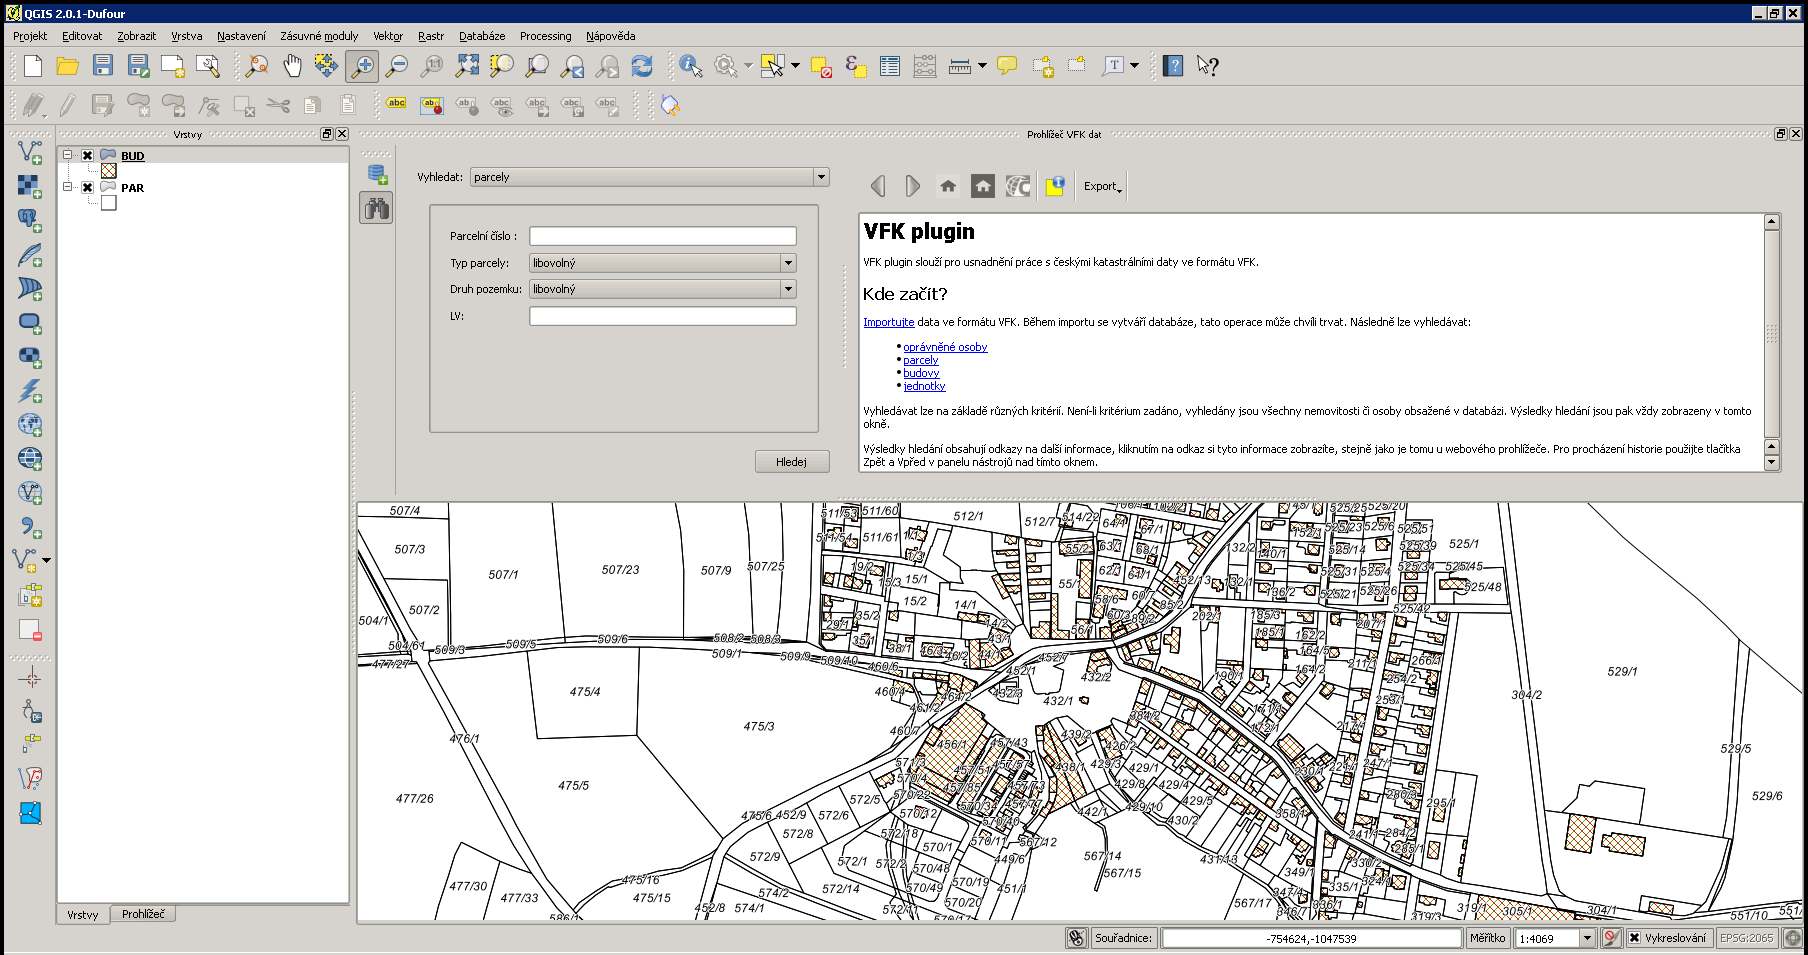
\includegraphics[width=\textwidth]{images/vfkPlugin-puvodni_okno.png}
\caption[VFK Plugin -- C++ verze]{VFK Plugin -- C++ verze (zdroj: \cite{cvut_vfkPlugin})}
\end{figure}

\newpage
\section{Funkcionalita}
Cílem zásuvného modulu je zjednodušit práci s~daty katastru
nemovitostí. Plugin byl proto navržen tak, aby byl schopen jednoduše
a~rychle řešit základní úlohy nad těmito daty. Mezi základní
funkcionalitu patří možnost vyhledávání podle:

\begin{itemize}
 \item vlastníků,
 \item parcel,
 \item budov,
 \item jednotek.
\end{itemize}

\begin{figure}[htb]
    \centering
    \begin{subfigure}[b]{0.4\textwidth}
        \centering
        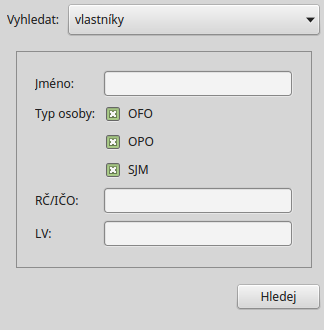
\includegraphics[width=\textwidth]{images/vfkPlugin-vlastnici.png}
        \caption{Vyhledávání vlastníků}
    \end{subfigure}
    ~
    \begin{subfigure}[b]{0.4\textwidth}
        \centering
        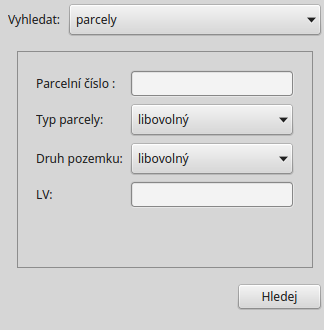
\includegraphics[width=\textwidth]{images/vfkPlugin-parcely.png}
        \caption{Vyhledávání parcel}
    \end{subfigure}
    \caption{Vyhledávací formuláře 1/2}
    \label{l_vyhledavani_1}
\end{figure}

\begin{figure}[htb]
    \centering
    \begin{subfigure}[b]{0.393\textwidth}
        \centering
        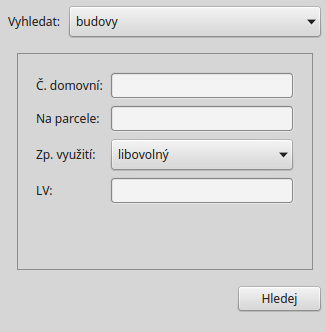
\includegraphics[width=\textwidth]{images/vfkPlugin-budovy.png}
        \caption{Vyhledávání budov}
    \end{subfigure}
    ~
    \begin{subfigure}[b]{0.4\textwidth}
        \centering
        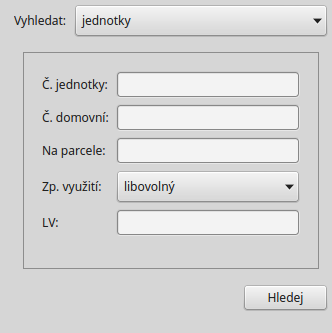
\includegraphics[width=\textwidth]{images/vfkPlugin-jednotky.png}
        \caption{Vyhledávání jednotek}
    \end{subfigure}
    \caption{Vyhledávací formuláře 2/2}
    \label{l_vyhledavani_1}
\end{figure}

Ve vedlejším okně, prohlížeči dat, se zobrazují výsledky
vyhledávání. Tato data lze interaktivně procházet, podobně jako je
tomu ve webovém prohlížeči, jelikož jsou ukládána ve formě HTML
stránek. Jsou zde implementovány základní vlastnosti HTML. Pro
navigaci mezi jednotlivými prvky jsou používány hypertextové
odkazy. Obsah okna prohlížeče je ukládán do historie, což usnadňuje
uživateli vyhledávání stále se opakujících informací (není potřeba
opakovaně provádět stejný databázový dotaz). Historii lze procházet
pomocí tlačítek \texttt{Vpřed} a~\texttt{Zpět}.

Pro zjištění aktuálního stavu o~dané nemovitosti je zde implementováno
propojení s~aplikací \textbf{Nahlížení do katastru
  nemovitostí}\footnote{http://nahlizenidokn.cuzk.cz/}.

Veškeré výpisy zobrazené v~prohlížeči zásuvného modulu lze exportovat,
a~to do následujících formátů:

\begin{itemize}
 \item \textbf{HTML}: umožňuje následné zobrazení ve webovém prohlížeči, případně import do textového procesoru,
 \item \textbf{zdrojový kód \latex}: umožňuje vytvoření PDF nebo PS.
\end{itemize}

Zásuvný modul a~mapové okno QGIS jsou navzájem propojené. Je tedy
možné v~mapovém okně zobrazit polohu vyhledaných prvků a~opačně
vyhledat informace o~prvcích, které byly vybrány pomocí nástroje
výběru QGIS právě v~mapovém okně.

Uživatelská přívětivost používání zásuvného modulu je zvýšena
\uv{dokovatelností} samotného okna pluginu. Modul je primárně ukotven
k~horní liště okna QGIS, ale je možné ho ukotvit i~k~ostatním
okrajům. Okno modulu lze samozřejmě používat i~samostatně
(neukotvené).

Pro vrstvy parcel (\texttt{PAR}) a~budov (\texttt{BUD}) byl vytvořen
předdefinovaný vzhled ve formátu \textit{.xml}, respektive
\textit{.qml}, se kterým QGIS nativně pracuje.

Součástí zásuvného modulu je také stručná nápověda, která je po
spuštění pluginu zobrazena stejně jako veškeré hledané informace
v~prohlížeči dat ve formátu HTML. Nápověda může být vyvolána i~po
kliknutí na příslušné tlačítko v~liště panelu nástrojů VFK
Pluginu. \cite{cvut_vfkPlugin}

\newpage
\section{Použití pluginu}

\subsection{Instalace a~spuštění}
Stávající zásuvný modul, který je napsán v~jazyce C++, je možné pod
operačním systémem Ubuntu nainstalovat dle skriptů dostupných na
stránkách
pluginu\footnote{http://freegis.fsv.cvut.cz/gwiki/VFK\_/\_QGIS\_plugin}. Pro
spuštění pod operačním systémem Windows, je potřeba stáhnout
předkompilovanou verzi pro danou verzi QGIS a~tu překopírovat do
požadovaného adresáře. Podrobný návod je uveden opět na stránkách
zásuvného modulu.

Takto nainstalovaný modul lze potom vyhledat v~QGIS v~nabídce Pluginy
$\rightarrow$ Spravovat zásuvné moduly. Zde lze plugin dohledat po
zadání filtru \textit{VFK}. Spuštění pluginu je poté možné z~hlavní
nabídky QGIS Pluginy $\rightarrow$ VFK Plugin $\rightarrow$ VFK
Plugin, nebo pomocí ikonky přímo z~nástrojové lišty.

\subsection{Rozložení}
Okno zásuvného modulu se skládá ze tří hlavních částí. Vlevo se
nachází hlavní panel nástrojů pro přepínání oken pro import souborů
VFK a~pro vyhledávání. Naprostou většinu pravé části tvoří prohlížeč
dat, ve kterém se zobrazují výsledky vyhledávání a~nápověda. Nad ním
je poté nástrojová lišta, která obsahuje nástroje pro práci se
zásuvným modulem.

\subsection{Načítání dat}
Pomocí zásuvného modulu je možné nahrát soubor VFK. Tento import je
k~dispozici pomocí tlačítka \uv{Procházet} v~nabídce \textit{Import
  VFK}. V~tomto okně je dále možné zvolit, které vrstvy se budou
importovat (PAR, BUD). V~případě, kdy není zatrženo ani jedno pole,
tak se načtou pouze popisná data. Bude tedy dostupné pouze vyhledávání
bez interakce s~mapovým oknem.

\subsection{Vyhledávání}
Po úspěšném načtení dat je zpřístupněno vyhledávání. Veškeré informace
vyhledané o~vlastnících, parcelách, budovách nebo jednotkách lze
pohodlně procházet pomocí hypertextových odkazů v~prohlížeči
dat. Náhled vyhledaných informací je uveden na obrázku
č. \ref{l_informace_o_parcele}.

\begin{figure}[htb]
\centering
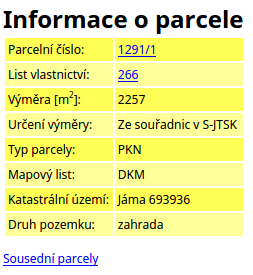
\includegraphics[width=0.4\textwidth]{images/vfkPlugin-informace_o_parcele.png}
\caption[Ukázka vyhledaných informací k~dané parcele]{Ukázka vyhledaných informací k~dané parcele}
\label{l_informace_o_parcele}
\end{figure}



% ==================================================================================
\clearpage
\chapter{Rozšíření stávající funkcionality}
\label{l_rozsireni_funkcionality}
V~této kapitole bych se chtěl postupně věnovat jednotlivým krokům,
které vedly k~rozšíření stávajícího zásuvného modulu programu QGIS
o~podporu zpracování změnových vět souborů VFK. Spolu s~tímto byly do
pluginu přidány další funkcionality, jež jsou zmíněny na následujících
řádcích kapitoly.

\section{Usnadnění distribuce pluginu}
Jak už bylo zmíněno v~kapitolách uvedených výše, stávající zásuvný modul byl napsán v~jazyce C++. Což znamená, že před prvním použitím se musí plugin překompilovat. 

Kompilace pod operačním systémem Linux (Ubuntu) může být provedena
pomocí skriptů\footnote{Návod dostupný na:
  http://freegis.fsv.cvut.cz/gwiki/VFK\_/\_QGIS\_plugin}, které
vytvořili autoři původní verze modulu.

Pod operačním systémem Microsoft Windows je situace poněkud
komplikovanější. Pro každou verzi programu QGIS musí být plugin
zkompilován samostatně vzhledem k~typu operačního systému
(32bit/64bit). Předkompilované verze mohou být staženy opět na
stránkách pluginu, avšak nejsou zde uvedeny veškeré verze QGIS jak pro
32bit systém, tak pro 64bit systém. Uživatel jiné verzi QGIS (jiného
typu operačního systému) by si tedy musel plugin zkompilovat sám, což
může být pro nezkušené uživatele značná překážka.

Výše zmíněné problémy značně snižují jak možnost většího rozšíření
zásuvného modulu, tak komfort při jeho instalaci
(aktualizaci). Řešením je přepis modulu do jazyka Python, čímž se
plugin stane snadněji dostupným pro všechny uživatele bez rozdílu
operačního systému, či verze programu QGIS.

\subsection{Přepis do jazyka Python}
Přepis zásuvného modulu do jazyka Python byl zásadním bodem této
práce. Při přepisu jsem se snažil kód vytvářet co možná nejvíce
podobný původnímu kódu v~jazyku C++, a~to hlavně z~důvodu, aby byly
zachovány veškeré funkcionality a~vlastnosti tak, jak jsou známé
stávajícím uživatelům nástroje.

Základní struktura kódu zásuvného modulu byla vygenerována pomocí
doporučovaného nástroje \textbf{Plugin
  Builder}\footnote{http://g-sherman.github.io/Qgis-Plugin-Builder/}
dostupného přímo z~QGIS. Přepis byl značně ulehčen díky použití stejné
knihovny Qt (respektive PyQt verze 4). V~následujících ukázkách je
porovnán původní kód v~jazyce C++ (ukázka č. \ref{l_loadLayerC++})
s~mnou napsaným kódem v~jazyce Python (ukázka
č. \ref{l_loadLayerPython}). Oba kódy slouží pro přidání vektorové
vrstvy ze souboru VFK do okna QGIS.

\begin{lstlisting}[style=c++, 
		    caption=Kód pro načtení vektorové vrstvy v~C++, 
		    label=l_loadLayerC++]
 void VfkMainWindow::loadVfkLayer( QString vfkLayerName )
{
  QgsDebugMsg( QString( "Loading vfk layer %1" ).arg( vfkLayerName ) );
  if ( mLoadedLayers.contains( vfkLayerName ) )
  {
    QgsDebugMsg( QString( "Vfk layer %1 is already loaded" ).arg( vfkLayerName ) );
    return;
  }
  QString composedURI = mLastVfkFile + "|layername=" + vfkLayerName;
  QgsVectorLayer *layer = new QgsVectorLayer( composedURI, vfkLayerName, "ogr" );
  mLoadedLayers.insert( vfkLayerName, layer->id() );
  setSymbology( layer );

  QList<QgsMapLayer *> myList;
  myList << layer;
  QgsMapLayerRegistry::instance()->addMapLayers( myList );
}
\end{lstlisting}

\newpage
\begin{lstlisting}[style=python, 
		    caption=Kód pro načtení vektorové vrstvy v~jazyce Python,
		    label=l_loadLayerPython]
def __loadVfkLayer(self, vfkLayerName):
  """
  Method loads VFK layer.
  :type vfkLayerName: str
  """
  qDebug("\n(VFK) Loading vfk layer {}".format(vfkLayerName))
  if vfkLayerName in self.__mLoadedLayers:
      qDebug(
	  "\n(VFK) Vfk layer {} is already loaded".format(vfkLayerName))
      return

  composedURI = self.__mDataSourceName + "|layername=" + vfkLayerName
  layer = QgsVectorLayer(composedURI, vfkLayerName, "ogr")
  if not layer.isValid():
      qDebug("\n(VFK) Layer failed to load!")

  self.__mLoadedLayers[vfkLayerName] = layer.id()

  try:
      self.__setSymbology(layer)
  except VFKWarning as e:
      QMessageBox.information(self, 'Load Style', e, QMessageBox.Ok)

  QgsMapLayerRegistry.instance().addMapLayer(layer)
\end{lstlisting}

\subsection{Instalace zásuvného modulu v~QGIS}
Díky přepisu zásuvného modulu do jazyka Python je plugin v~QGIS
dostupný standardním způsobem, jako ostatní pluginy napsány v~tomto
jazyce. Plugin v~současné době není dostupný v~oficiálním repositáři
QGIS. Pro instalaci pluginu je potřeba do QGIS přidat nový repositář
spravovaný organizací
OSGeoREL\footnote{http://geomatics.fsv.cvut.cz/research/osgeorel/},
pod kterou je tento plugin vyvíjen. Repositář je dostupný na adrese
\url{http://geo.fsv.cvut.cz/osgeorel/qgis-plugins.xml}, viz
obr. \ref{l_repo_detail}. Modul je šířený jako experimentální, proto
musí být tato volba zohledněna při jeho instalaci, viz
obr. \ref{l_qgis_plugins}. Okno pro zadání repositáře vyvoláme
v~záložce \textit{Plugins} $\rightarrow$ \textit{Manage and install
  plugins}.

\begin{figure}[htb]
\centering
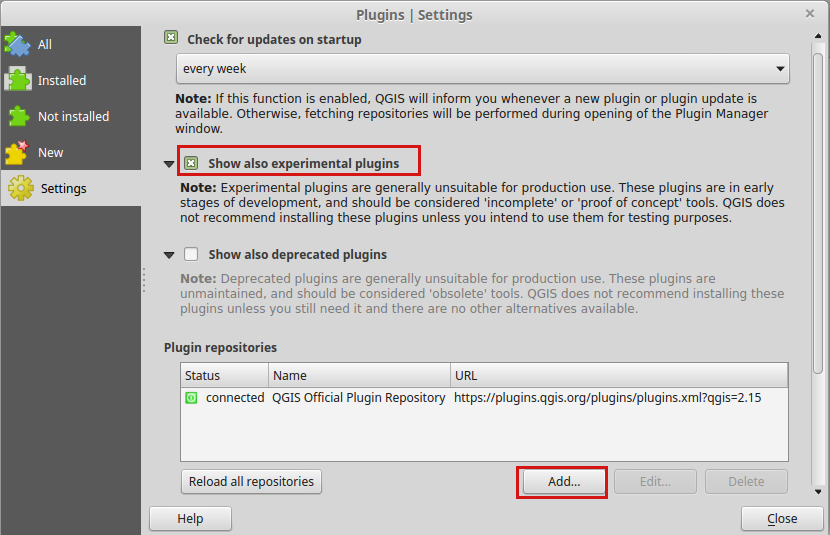
\includegraphics[width=1\textwidth]{images/qgis_repo_plugins.png}
\caption[Přidání repositáře QGIS]{Přidání repositáře QGIS}
\label{l_qgis_plugins}
\end{figure}

\begin{figure}[htb]
\centering
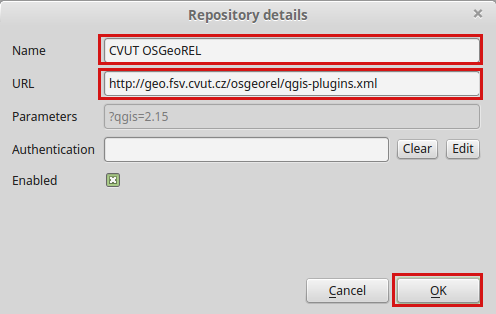
\includegraphics[width=0.5\textwidth]{images/qgis_repo_detail.png}
\caption[Přidání repositáře QGIS -- detail]{Přidání repositáře QGIS -- detail}
\label{l_repo_detail}
\end{figure}

Po přidání repositáře a~jeho aktualizaci je zásuvný modul dohledatelný
standardním způsobem pod názvem \textbf{VFK Plugin}, viz
obr. \ref{l_qgis_hledani_pluginu}.

\begin{figure}[htb]
\centering
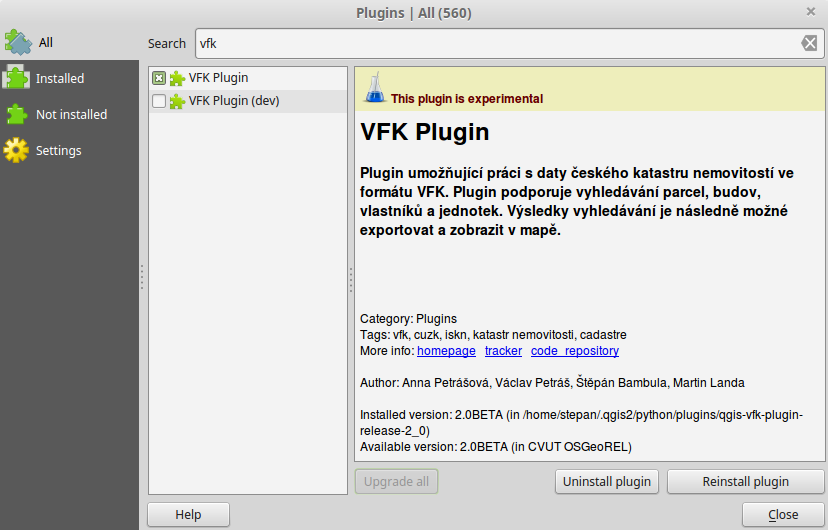
\includegraphics[width=1\textwidth]{images/qgis_plugin_vyhledani.png}
\caption[Vyhledání zásuvného modulu]{Vyhledání zásuvného modulu}
\label{l_qgis_hledani_pluginu}
\end{figure}

Po správné instalaci zásuvného modulu se do nástrojové lišty přidá
jeho ikonka (viz obr. \ref{l_plugin_ikona}). Plugin je poté dostupný
po kliknutí na tuto ikonku nebo z~menu \textit{Plugins} $\rightarrow$
\textit{VFK} $\rightarrow$ \textit{Otevřít prohlížeč VFK}.

\begin{figure}[H]
\centering

\includegraphics[scale=0.9]{images/vfkPluginIcon.png}
\caption[VFK Plugin -- ikona]{VFK Plugin -- ikona}
\label{l_plugin_ikona}
\end{figure}

% -----------------------------------------------------------------------
\clearpage
\section{Úprava GDAL VFK driveru}
\label{l_uprava_gdal}
Před začátkem práce na podpoře zpracování změnových vět v~QGIS VFK
Pluginu bylo potřeba provést několik nezbytných úprav na straně GDAL
VFK driveru, který plugin využívá pro čtení dat VFK, respektive jejich
zápis do databáze SQLite.

Úprava byla provedena ve spolupráci s~autorem GDAL VFK driveru
Martinem Landou, který provedl většinu změn ovladače, které byly pro
zpracování změnových VFK souborů nezbytné.

Veškeré provedené změny na ovladači VFK budou dostupné v~knihovně GDAL
od verze 2.2.0, v~současné době jsou dostupné ve formě \uv{patche},
který je obsahem CD přiloženého k~diplomové práci. Tento \uv{patch} je
vytvořen proti vývojové verzi 2.2.0 knihovny GDAL.

\subsection{Načítání dat z~více souborů}
Vzhledem ke struktuře, v~jaké jsou změnová data dodávána od ČUZK
uživatelům, musela být implementována podpora načítání několika VFK
souborů do jedné SQLite databáze. VFK soubory jsou k~uživatelům
distribuovány ve struktuře, která je uvedena v~následující ukázce
č. \ref{l_struktura_sireni_vfk}.

\begin{figure}[htb]
\centering
\begin{minipage}{0.9\textwidth}
  \dirtree{%
  .1 /.
  .2 nemodebo.
  .3 vfk\_soubor.vfk.
  .2 nvfpkmbpej.
  .3 vfk\_soubor.vfk.
  .2 \vdots.
  }
\end{minipage}
\caption{Struktura VFK souborů}
\label{l_struktura_sireni_vfk}
\end{figure}

K~tomuto byla upravena funkce pro načítání dat. Původní chování VFK
driveru bylo, že při prvním čtení VFK souboru se na pozadí ve stejném
adresáři vytvořila databáze SQLite (její název byl shodný s~názvem
vstupního souboru), do které byla data načtena. Při opakovaném čtení
VFK souboru se stejným názvem, se data četla již z~existující
databáze. Jméno výstupní SQLite databáze mohlo být ovlivněno pomocí
proměnné prostředí \texttt{OGR\_VFK\_DB\_NAME}, data poté byla
ukládána/načítána do/z této databáze.

Nebylo tedy možné zpracovat data, která jsou uložena v~adresářové
struktuře (viz ukázka \ref{l_struktura_sireni_vfk}), kdy jsou některé
VFK bloky uloženy v~jednom adresáři a~další ve druhém pod stejným
názvem souboru.

Chování driveru bylo proto opraveno tak, že pokud uživatel potřebuje
načíst více VFK souborů do jedné databáze, musí nejprve zadat cestu
k~výstupní SQLite databází pomocí proměnné prostředí
\texttt{OGR\_VFK\_DB\_NAME}. Při čtení prvního souboru se načtou data
standardním způsobem do databáze, ale při čtení dalších driver porovná
tabulky v~databázi s~datovými bloky čteného VFK souboru. Jestliže
tabulka daného jména v~databázi neexistuje, tak ji vytvoří a~pokračuje
v~načítání dat.

Při načítání dat driver testuje (viz \ref{l_gdal_kontrola_zmen}), zda
se jedná o~změnový, nebo stavový VFK soubor. Jestliže se jedná
o~stavový, tak driver nepovolí načítání dat, která jsou již v~databázi
uloženy (vznikaly by duplicity, což není u~stavových dat možné). Při
čtení změnového souboru je povoleno ukládání prvků s~\texttt{ID},
které je již v~tabulce uložené (ve změnovém souboru je možné uložit
prvky se stejným \texttt{ID}, viz kapitola
\ref{l_struktura_zmen}). Správné uložení prvků s~duplicitním
\texttt{ID} je zajištěno pomocí databázového indexu \texttt{UNIQUE},
který je vytvářen právě jen pro stavová data.

\begin{lstlisting}[style=c++, 
		    caption={Výňatek z~kódu pro kontrolu změnového souboru}, 
		    label=l_gdal_kontrola_zmen]
else if (pszLine[1] == 'H') {
    /* check if amendment file */
    if (EQUAL(pszLine, "&HZMENY;1")) {
	m_bAmendment = TRUE;
    }

    /* header - metadata */
    AddInfo(pszLine);
}
\end{lstlisting}

\subsection{Čtení z~databáze SQLite}
Další podstatnou změnou na VFK driveru knihovny GDAL bylo přidání
podpory pro čtení z~databáze SQLite. Díky této nové funkcionalitě je
možné v~QGIS načíst vrstvy z~databáze, do které byly aplikovány změny.

\subsection{Vytváření geometrie prvků}
Vytváření geometrie pro jednotlivé prvky, které jsou obsaženy ve VFK
souboru, se děje pomocí metody \texttt{int
  IVFKDataBlock::LoadGeometry()}. V~dosavadní verzi VFK driveru byla
tato metoda volána při požadavku o~konkrétní prvek (například pomocí
konzolového příkazu: \texttt{ogrinfo Export\_vse.vfk PAR -FID
  1}). Geometrie tedy nebyla sestavena dopředu po uložení dat do
databáze, ale až poté, co si uživatel o~daný prvek přímo zažádal.

Toto chování muselo být vzhledem ke struktuře, v~jaké se k~uživatelům
dostávají VFK soubory, změněno. Geometrie se nyní sestavuje ihned po
načtení dat do databáze. Jestliže databáze neobsahuje potřebné tabulky
pro její sestavení, tak je zobrazeno upozornění\footnote{Upozornění,
  že v~databázi chybí tabulka \texttt{HP}, potřebná pro sestavení
  geometrie parcel:\\\uv{Warning 3: Data block HP not found. Unable to
    build geometry for PAR.}}. Při čtení dalšího VFK souboru jsou data
ukládána do stejné databáze a~po jejich uložení se opět testuje, zda
jsou k~dispozici veškeré potřebné tabulky pro sestavení geometrie
prvků. Jestliže ano, tak je geometrie sestavena. V~opačném případě je
opět zobrazeno upozornění.

\subsection{Implementace na straně zásuvného modulu}
Výše uvedené změny týkající se v~načítání vícero VFK souborů do stejné
databáze byly implementovány i~do zásuvného modulu. Spolu s~touto
změnou byla do zásuvného modulu přidána i~možnost načíst přímo SQLite
databáze s~VFK daty.

Tato rozšířená funkcionalita je do zásuvného modulu přidána pouze
v~případě, kdy je na počítači uživatele dostupná knihovna GDAL od
verze \texttt{2.2.0}. V~případě nižší verze je aktualizován popisek
ikonky pro přidání dalších VFK souborů (viz
\ref{l_kontrola_verze_gdal}) a~přidání dalších souborů není umožněno.

\begin{lstlisting}[style=python, 
		    caption={Kontrola verze GDAL na straně VFK pluginu}, 
		    label=l_kontrola_verze_gdal]
if gdal_version < 2020000:
    self.pb_nextFile.setEnabled(False)
    self.pb_nextFile.setToolTip(
	u'Neni mozne nacist vice souboru, verze GDAL je nizsi nez 2.2.0.')
\end{lstlisting}

Jak z~výše uvedených vět vyplývá, k~přidání této funkcionality musel
být změněn i~vzhled samotného okna zásuvného modulu pro načítání
dat. Nový vzhled je uveden na obrázku
č. \ref{l_plugin_novy_vzhled}. Kde byly přidány následující prvky:

\begin{enumerate}
 \item Tlačítko pro vložení nového řádku do formuláře pro přidání souboru,
 \item nově vygenerovaný formulář pro vyhledání VFK souboru,
 \item indikátor stavu načítání VFK souborů.
 \item popisek stavu načítání dat.
\end{enumerate}

\begin{figure}[htb]
\centering
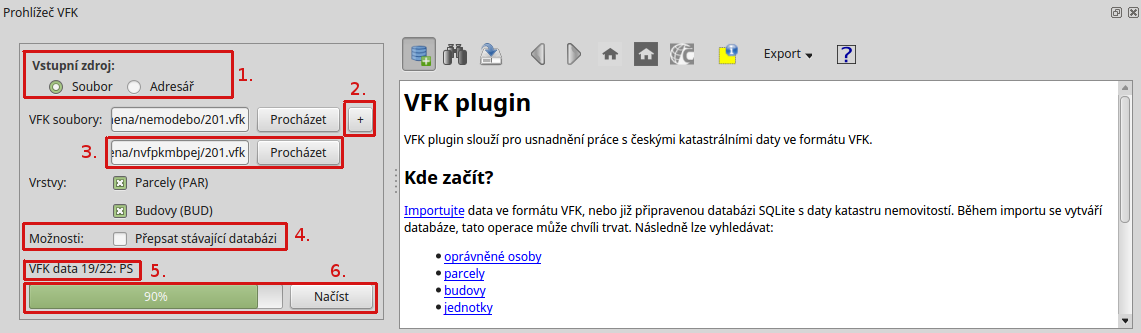
\includegraphics[width=0.9\textwidth]{images/vfkPlugin-novy_vzhled.png}
\caption[VFK Plugin -- okno pro načítání souborů]{VFK Plugin -- okno pro načítání souborů}
\label{l_plugin_novy_vzhled}
\end{figure}


\newpage
% -----------------------------------------------------------------------
\section{Zpracování změnových vět}
\label{l_zpracovani_zmen}
Schopnost umět zpracovat změnové věty VFK souborů je důležitá pro
každého uživatele, který s~daty katastru nemovitostí pracuje. Jestliže
uživatel již jednou vlastní stavová data pro dané území a~potřebuje
hlídat aktuálnost těchto dat, je pro něj výhodnější stahovat právě
změnové VFK soubory, než soubory stavové.

Zpracování těchto vět pomocí zásuvného modulu v~QGIS nebylo do této
doby možné. O~implementaci podpory pro jejich zpracování na straně VFK
pluginu pojednává právě tato kapitola.

Změnové věty jsou směrem k~uživatelům šířeny ve stejné struktuře jako
stavová data, viz obr. \ref{l_struktura_sireni_vfk}. Pro jejich
zpracování musely být nejprve provedeny úpravy na straně VFK driveru
v~knihovně GDAL, viz kapitola \ref{l_uprava_gdal}. Díky tomuto kroku
a~úpravě principu načítání souborů v~okně zásuvného modulu (viz
obr. \ref{l_plugin_novy_vzhled}) je možné změnové VFK soubory uložit
do jedné databáze a~pomocí VFK pluginu zobrazit v~programu
QGIS. V~případě, kdy změny obsahují potřebné datové bloky, je nad
změnovými daty umožněno i~vyhledávání.

\subsection{Metodika aplikace změn na stavová data}
Aplikace změn na stavová data předpokládá, že uživatel již má pomocí
VFK driveru knihovny GDAL připravenou databázi jak se stavovými daty,
tak s~daty změnovými. V~opačném případě může uživatel tyto databáze
vytvořit pomocí samotného VFK pluginu.

Pro aplikaci změn byla vytvořena samostatná třída
(\texttt{ApplyChanges}), pomocí které mohou být změny aplikovány. Toto
může být provedeno jednak pomocí zásuvného modulu (viz
\ref{l_implementace_zmen}), nebo pomocí samostatně spustitelné
konzolové aplikace (viz \ref{l_apply_changes_ukazka}).

Vstupními argumenty pro tuto třídu, respektive metodu
\texttt{run(\dots)}, jsou:

\begin{itemize}
 \item \textbf{Hlavní databáze:} Databáze, která obsahuje stavová data, na něž budou změny aplikovány.
 \item \textbf{Změnová databáze:} Databáze obsahující změnová data.
 \item \textbf{Režim \uv{debug}:} Nepovinný argument. V~případě jeho
   zadání jsou na standardní výstup vypisovány veškeré SQL příkazy do
   databáze. Implicitně je nastaven na hodnotu \texttt{False}.
\end{itemize}

Jediným výstupním argumentem je poté cesta k~nově vytvořené databázi, která bude obsahovat stavová data s~aplikovanými změnami.

% \newpage
\begin{lstlisting}[caption={Nápověda ke konzolové aplikaci pro implementaci změn}, 
		    label=l_apply_changes_ukazka]
$ ./applyChanges.py -h

usage: applyChanges.py [-h] [-v] -m MAIN -c CHANGES -e EXPORT [-d]

Script applies changes from amendment VFK database to main VFK database. In this process new database is created.

optional arguments:
  -h, --help            show this help message and exit
  -v, --version         show program's version number and exit
  -d, --debug           Enables debug mode.
  -m MAIN, --main MAIN  Path to the main database.
  -c CHANGES, --changes CHANGES
                        Path to the database with changes.
  -e EXPORT, --export EXPORT
                        Path to the new database which will be created.
\end{lstlisting}

V~prvním kroku se pomocí nástroje \texttt{shutil.copy2(src, dst)}
vytvoří kopie hlavní databáze. Cesta k~ní je zadána pomocí výstupního
argumentu. Čas potřebný pro tvorbu kopie databáze je přímo úměrný její
velikosti. Tento krok proto může být pro objemná data časově
náročný. Díky tvorbě kopie a~práce s~ní je ale zajištěno, že
v~případě, kdyby se aplikace změn nepovedla, uživatel nepřijde
o~původní data.

V~dalším kroku se příkazem \texttt{sqlite3.connect(database)} provede
připojení ke kopii databáze (v~dalším textu bude tato kopie označována
jako hlavní / \uv{main}). Databáze se změnami je poté k~této hlavní
databázi připojena pomocí SQL příkazu \texttt{ATTACH
  DATABASE}\footnote{https://www.sqlite.org/lang\_attach.html}. Práce
s~takto připojenou databází je poté shodná jako se schématy, známými
například z~PostgreSQL.

Samotné změny jsou aplikovány pouze z~tabulek, které podporují princip
\uv{historizace} (viz kapitola \ref{l_struktura_zmen}) a~které nejsou
prázdné. Tyto tabulky musí obsahovat sloupec \texttt{STAV\_DAT}. Pro
výběr odpovídajících tabulek slouží k~tomu určená metoda
\texttt{\_\_findTablesWithChanges(self)}.

Při aplikaci změn jsou v~cyklu pro každou tabulku spouštěny databázové
příkazy \texttt{DELETE} (viz ukázka \ref{l_changes_delete})
a~\texttt{INSERT} (viz ukázka \ref{l_changes_insert}), kde proměnná
\texttt{table} označuje jméno databázové tabulky, proměnná
\texttt{column} jméno příslušného sloupce, \texttt{columns} označuje
seznam sloupců a~proměnná \texttt{id} je nahrazena identifikátorem
vkládaného prvku z~databáze, která obsahuje změnová data.

Příkaz \texttt{DELETE} z~hlavní databáze smaže veškeré prvky, které se
vyskytují v~databázi se změnovými daty. Tento příkaz je vykonán,
protože v~databázi se změnovými daty jsou vždy aktuálnější informace
o~prvcích, než v~databázi původní.

\begin{lstlisting}[style=sql, caption={Aplikace změn -- příkaz DELETE}, 
		    label=l_changes_delete]
DELETE FROM main.{table}
WHERE id IN (
SELECT DISTINCT t1.id FROM main.{table} t1
JOIN db2.{table} t2 ON t1.id = t2.id);
\end{lstlisting}

\begin{lstlisting}[style=sql, 
		    caption={Aplikace změn -- příkaz INSERT}, 
		    label=l_changes_insert]
INSERT INTO main.{table}
SELECT {columns} FROM db2.{table}
WHERE ogr_fid={selected_ogr_fid}
  AND stav_dat=0
  AND id = {id};
\end{lstlisting}

Po smazání veškerých neaktuálních záznamů z~hlavní databáze, je
vykonán příkaz \texttt{INSERT}. Tento příkaz je spuštěn v~cyklu nad
všemi záznamy ze změnové databáze, které jsou určeny pro
import. V~případě, kdy jsou ve změnové databázi prvky, na kterých bylo
v~exportovaném období použito více operací (UPDATE, INSERT, DELETE),
jsou příslušné prvky seřazeny podle data vzniku a~do databáze je
vkládán pouze nejnovější prvek (ten je jednoznačně vybrán dle
identifikátoru \texttt{selected\_ogr\_fid}).

Pro lepší orientaci o~průběhu aplikování změn na stavová data byl vytvořen diagram, viz obr. \ref{l_zmeny_diagram}.

\begin{figure}
  \centering
  \includestandalone[mode=buildnew, height=0.7\paperheight]{diagram}
  \caption{Diagram průběhu implementace změn na stavová data}
  \label{l_zmeny_diagram}
\end{figure}


\newpage
\subsection{Implementace na straně zásuvného modulu}
\label{l_implementace_zmen}
Funkcionalita pro aplikování změn z~prostředí zásuvného modulu byla
implementována díky vytvoření nového formuláře v~okně pluginu. Na okně
zásuvného modulu byly provedeny následující úpravy:

\begin{enumerate}
 \item \textbf{Ikona změn:} Okno pro aplikaci změn na stavová data je vyvoláno pomocí nově vytvořené ikony v~nástrojové liště, viz obr. \ref{l_ikona_zmen}.

\begin{figure}[htb]
\centering

\includegraphics[scale=0.9]{images/applyChanges.png}
\caption[VFK Plugin -- ikona pro zpracování změn]{VFK Plugin -- ikona pro zpracování změn}
\label{l_ikona_zmen}
\end{figure} 
 
\item \textbf{Formuláře:} K~dispozici jsou tři formuláře pro zadání
  cesty ke vstupní databázi se stavovými daty, k~databázi se změnovými
  daty a~databázi výstupní, do které budou uložena stavová data
  s~aplikovanými změnami.
 
\item \textbf{Popisek průběhu zpracování:} V~tomto popisku jsou
  zobrazovány informace o~průběhu zpracování změn.
 
\item \textbf{Grafický indikátor průběhu:} Zde je průběh zpracování
  změn vyjádřen procentuálně a~graficky.
 
\item \textbf{Tlačítko pro zpracování:} Po stisku tohoto tlačítka je
  je vyvolána metoda \texttt{run(\dots)}, díky které jsou změny
  aplikovány do databáze se stavovými daty.
 
\end{enumerate}

Funkcionalita pro aplikaci změn obsažených v~databázi SQLite na data
obsažená v~databázi se stavovými daty je do zásuvného modulu přidána
pouze v~případě, kdy je na počítači uživatele dostupná knihovna GDAL
ve verzi \texttt{2.2.0} a~vyšší. V~opačném případě je ikonka pro
zpracování změn neaktivní.

\begin{figure}[htb]
\centering
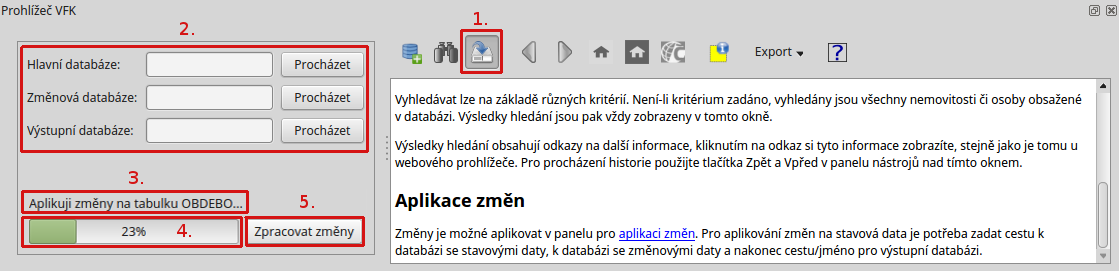
\includegraphics[width=0.9\textwidth]{images/vfkPlugin-zmeny.png}
\caption[VFK Plugin -- okno pro zpracování změn]{VFK Plugin -- okno pro zpracování změn}
\label{l_plugin_zmeny}
\end{figure}


% -----------------------------------------------------------------------
\clearpage
\section{Popis tříd zásuvného modulu}

\subsubsection{ApplyChanges}
Třída, která se stará o~aplikaci změn, které jsou pomocí \texttt{VFK
  Driveru GDAL} uloženy do databáze SQLite, na SQLite databázi
vytvořenou ze stavového VFK souboru. Podrobnější popis zpracování
změnových souborů touto třídou je k~dispozici v~kapitole
\ref{l_zpracovani_zmen}.

\subsubsection{BudovySearchForm}
Jedná se o~třídu, která se stará o~vyhledávací prvky ve formuláři pro
vyhledávání budov. Třída dědí od třídy \texttt{QWidget}. Vzhled
uživatelského rozhraní této třídy byl navržen samostatně pomocí
programu \texttt{Qt Designer}. Kód návrhu je uložen v~souboru
\texttt{ui\_budovysearchform.ui}, respektive v~překompilované verzi
pro jazyk Python \texttt{ui\_budovysearchform.py}. Ukázka konstruktoru
třídy je uvedena v~příloze \ref{l_budovySearchForm_konstruktor}.

\subsubsection{DocumentBuilder}
V~třídě \texttt{DocumentBuilder} se sestavuje dokument, který bude
zobrazen v~prohlížeči dat (nebo exportován do některého
z~podporovaných formátů), na základě výsledků vyhledávání. O~správné
sestavení se stará metoda \texttt{buildHtml}, viz příloha
\ref{l_buildHtml}.

Třída mimo jiné obsahuje několik metod pro správné sestavení tabulek
(např. \texttt{tableParcely(self, model, parIds, LVColumn)}), metody
pro tvorbu jednotlivých částí listu vlastnictví
(např. \texttt{partTelesoB1(self, parIds, budIds, jedIds, opsubIds,
  forLV)}), nebo metody pro zobrazení detailu o~vyhledávaném tělese
(např. \texttt{pageBudova(self, id)}).

Důležitou metodou v~této třídě je metoda \texttt{pageHelp(self)}, díky
které je možné zobrazit krátkou nápovědu k~zásuvnému modulu, a~metoda
\texttt{saveDefinitionPoint( self, id, nemovitost)}, která slouží
k~získání a~uložení definičního bodu vyhledané nemovitosti.

\subsubsection{Domains}
V~této třídě jsou jednoduché metody pro zjištění domény prvku na
základě vstupního argumentu. Je zde metoda \texttt{anoNe(an)}, která
testuje, zda je vstupní argument rovný \uv{a}, a~podle toho vrací
\texttt{True/False}. Metoda \texttt{cpCe(kod)} převádí hodnotu
vstupního argumentu na řetězec \uv{Číslo popisné} / \uv{Číslo
  evidenční}. Metoda \texttt{druhUcastnika(kod)} kontroluje, o~jaký
typ subjektu se jedná (např. právnická osoba). Poslední metodou je
metoda \texttt{rodinnyStav(kod)}, která vrací rodinný stav subjektu na
základě zadaného vstupního kódu.

\subsubsection{HtmlDocument}
Třída \texttt{HtmlDocument} je potomkem třídy \texttt{VfkDocument}(viz
\ref{l_vfkDocument}). Jsou v~ní obsaženy metody pro tvorbu
jednotlivých částí kódu v~jazyce \textit{HTML}. Vhodnou kombinací
těchto částí je poté sestaven celý \textit{HTML} dokument. Takto
připravený dokument je poté možné vyexportovat pomocí příslušné
funkcionality a~zobrazit v~libovolném prohlížeči.

\subsubsection{JednotkySearchForm}
V~této třídě se řeší vyhledávání jednotek pomocí vyhledávacích
formulářů navržených v~programu \texttt{Qt Designer}. Vyhledávat lze
podle čísla jednotky, domovního čísla, čísla parcely, ke které
jednotka patří, listu vlastnictví nebo způsobu využití jednotky. Třída
je potomkem třídy \texttt{QWidget}.

\subsubsection{LatexDocument}
Třída \texttt{LatexDocument} obsahuje metody, pomocí nichž se vytváří
části kódu, které jsou nakonec sestaveny v~\latex~dokument. Takto
sestavený dokument je poté vyexportován pomocí příslušné funkcionality
modulu a~je připravený pro export například od formátu \textit{PDF}
(\texttt{pdflatex}). Třída dědí od rodičovské třídy
\texttt{VfkDocument}.

\subsubsection{MainApp}
Třída \texttt{MainApp} je stěžejní třídou zásuvného modulu. Dědí od
tříd \texttt{QDockWidget}, \texttt{QMainWindow}
a~\texttt{Ui\_MainApp}. Obsahuje metody pro načítání VFK souborů,
nastavuje symbologii načtených vrstev, propojuje vyhledávání s~mapovým
oknem QGIS, stará se o~exporty do definovaných formátů. Ve třídě se
také přidává funkcionalita jednotlivým prvkům zásuvného modulu.

\subsubsection{OpenThread}
Tato třída se stará o~načítání jednotlivých \textit{VFK} souborů
v~separátním vlákně. Díky použití jiného vlákna pro načítání souborů,
se práce se zásuvným modulem stává plynulejší. Třída dědí od třídy
\texttt{QThread} dostupné v~použité knihovně \texttt{PyQt4}. Obsahuje
jedinou metodu (\texttt{run(self)}) pro spuštění separátního vlákna,
jejíž předpis je dostupný v~příloze č. \ref{l_thread_run}.

\subsubsection{ParcelySearchForm}
Třída \texttt{ParcelySearchForm} stejně jako předešlé třídy pro
vyhledávání dědí od rodičovské třídy \texttt{QWidget}. Obsahuje
metody, které pracují s~navrženými grafickými prvky. Díky těmto
metodám je možné vyhledávat parcely podle parcelního čísla, typu
parcely, druhu pozemku nebo listu vlastnictví.

\subsubsection{RichTextDocument}
Třída se stará o~tvorbu \textit{HTML} dokumentu, který obsahuje
výsledky vyhledávání a~je zobrazen v~prohlížeči dat. Třída dědí od
rodičovské třídy \texttt{VfkDocument}.

\subsubsection{SearchFormController}
Třída \texttt{SearchFormController} získává hodnoty ze vstupních
formulářů, které jsou obsahem tříd pro vyhledávání
(\texttt{BudovySearchForm}, \texttt{JednotkySearchForm},
\texttt{Par\-celySearchForm}, \texttt{VlasniciSearchForm}). Z~těchto
vstupních hodnot poté sestavuje vyhledávací dotaz, který pomocí
signálu \texttt{actionTriggered} emituje dále. Ukázka kódu pro
sestavení vyhledávacího dotazu pro parcely je uvedena v~příloze
\ref{l_search_parcely}.

\subsubsection{VfkDocument}
\label{l_vfkDocument}
Jedná se o~abstraktní třídu, ze které jsou odvozeny třídy pro
sestavení dokumentů v~různých formátech (\texttt{HtmlDocument},
\texttt{LatexDocument}, \texttt{RichTextDocument}). Jsou zde
implementovány základní metody, které zajišťují správné sestavení
dokumentu.

\subsubsection{VfkPlugin}
Tato třída implementuje zásuvný modul do programu QGIS. Jsou zde
uvedeny metody, které vytvářejí instanci pluginu v~programu QGIS po
jeho instalaci, nebo metody, které tuto instanci ruší. Tato třída byla
vygenerována automaticky při tvorbě základního schéma pluginu
nástrojem \textit{Plugin Builder} a~později upravena dle konkrétních
potřeb.

\subsubsection{VfkTableModel}
Tato třída dědí od třídy \texttt{QSqlQueryModel}, která poskytuje
model pro čtení SQL dotazů. Třída komunikuje s~připojenou databází,
která je do třídy předávána pomocí argumentu
\texttt{connectionName}. Ke komunikaci jsou používány standardní SQL
dotazy, které jsou do databáze předávány metodou
\texttt{self.setQuery(query,
  QSqlDatabase.database(self.\_\_mConnectionName))}.

\subsubsection{VfkTextBrowser}
\texttt{VfkTextBrowser} je třída, která dědí od třídy
\texttt{QTextBrowser}. Třída byla stanovena jako \uv{zástupná} pro
prvek \texttt{vfkBrowser} v~okně zásuvného modulu. Tento prvek slouží
jako prohlížeč dat.

\subsubsection{VlastniciSearchForm}
Jedná se o~třídu, která slouží k~vyhledávání vlastníků podle jména,
typu (fyzická osoba, právnická osoba, společné jmění manželů), rodného
čísla (případně IČO) nebo listu vlastnictví. Metody třídy získávají
hodnoty vstupních polí / \uv{checkboxů}.


% -----------------------------------------------------------------------
\clearpage
\rhead{Závěr}       % vpravo název kapitoly
\chapter*{Závěr}
\addcontentsline{toc}{chapter}{Závěr}

Cílem diplomové práce bylo rozšířit stávající zásuvný modul pro práci
s~katastrálními daty v~programu QGIS. Samotnému rozšíření modulu
o~nové funkcionality předcházelo jeho přepsání do jazyka Python, díky
čemuž se velice usnadnila jeho distribuce směrem k~uživatelům. Hlavním
tématem diplomové práce bylo zpracování změnových vět výměnného
formátu katastru nemovitostí.

Práce byla rozdělena do dvou částí -- teoretické
a~praktické. V~teoretické části jsem se věnoval rešerši dostupných
nástrojů pro zpracování a~práci s~katastrálními daty a~použité
technologii, která byla nezbytná pro vypracování práce. Dále jsem zde
vypracoval kapitolu týkající se Informačního systému katastru
nemovitostí, ze kterého jsou datové soubory VFK exportovány. Především
jsem se zde ale zabýval výměnným formátem katastru nemovitostí. Zde
jsem kladl důraz na jeho strukturu, jejíž znalost je nezbytná pro
správnou funkcionalitu zásuvného modulu. V~kapitole jsem se zaměřil
i~na strukturu změnových vět VFK tak, aby mohl být vypracován hlavní
bod diplomové práce -- \textbf{zpracování změnových vět}.

Na teoretickou část volně navazuje kapitola týkající se stavu
současného zásuvného modulu pro zpracování katastrálních dat. Zde jsem
se snažil popsat práci s~modulem od jeho instalace a~zprovoznění pod
QGIS, přes načítání souborů VFK, až k~jeho klíčovým funkcionalitám
týkajících se samotného vyhledávání nad importovanými katastrálními
daty. Nechybí zde informace o~možnostech exportu výsledků vyhledávaní
do podporovaných formátů.

Ve stěžejní kapitole praktické části -- Rozšíření stávající
funkcionality (\ref{l_rozsireni_funkcionality}) -- jsem popsal veškerý
svůj přínos k~rozšíření zásuvného modulu. Jsou zde zmíněny kroky,
které vedly k~přepisu stávajícího modulu do jazyka Python, potřebné
změny na straně ovladače VFK v~knihovně GDAL, nově přidaná
funkcionalita týkající se zpracování změnových vět a~popis tříd
zásuvného modulu, pro rychlejší orientaci v~kódu.

Při přepisu stávajícího zásuvného modulu do jazyka Python jsem se
snažil držet co možná nejvíce původního kódu v~jazyce C++. Modul byl
navržen s~pomocí stejné knihovny Qt, respektive PyQt, která je jednou
z~hlavních knihoven pro tvorbu uživatelského rozhraní a~značně
ulehčuje tvorbu celé aplikace. Zásuvný modul komunikuje s~prostředím
QGIS díky použití aplikačního rozhraní QGIS API.

Poté, co byl stávající zásuvný modul přepsán, tak byl umístěn do nově
vzniklého
repositáře\footnote{\url{http://geo.fsv.cvut.cz/osgeorel/qgis-plugins.xml}},
který spravuje organizace OSGeoREL na ČVUT v~Praze. Zde je plugin
dostupný ve verzi \texttt{2.0BETA} a~jeho funkcionalita kopíruje
původní zásuvný modul v~C++. Pro tuto verzi modulu byla v~oficiálním
repositáři se zdrojovým
kódem\footnote{\url{https://github.com/ctu-osgeorel/qgis-vfk-plugin/tree/release-2_0}}
vytvořena nová vývojová větev \texttt{release-2\_0}. Modul je v~této
formě dostupný pro uživatele po přidání výše zmíněného repositáře do
programu QGIS.

Funkcionalitě týkající se zpracování změnových vět předcházela úprava
ovladače VFK v~knihovně GDAL. Zde bylo provedeno několik úprav. Jako
jedna z~nejdůležitějších může být zmíněna podpora načítání více
souborů do jedné databáze SQLite, či úprava struktury výstupní
databáze podle toho, zda je načten stavový, nebo změnový soubor
VFK. Další důležitou novou vlastností ovladače je možnost čtení přímo
z~databáze SQLite, čímž je možné do QGIS načíst databázi, na kterou
byly aplikovány změnové věty.

Pro zpracování změnových vět vznikla samostatná třída, která umožňuje
aplikovat změny, které jsou uloženy v~předem připravené databázi
SQLite, na stavová data, která opět musí být uložena v~předem
připravené SQLite databázi. Výstupem je nově vzniklá databáze s~již
obsaženými změnami. Změny mohou být aplikovány jednak pomocí vzniklé
konzolové aplikace, nebo přímo v~zásuvném modulu.

Nově vzniklé funkcionality jsou dostupné od verze \texttt{2.1BETA}
zásuvného modulu a~jsou k~dispozici pro všechny uživatele, kteří mají
nainstalovanou knihovnu GDAL ve verzi 2.2.0 a~vyšší. Vývoj této verze
probíhal (a~stále probíhá) ve větvi \texttt{master} opět na serveru
Github, kde jsou k~dispozici veškeré zdrojové kódy. Mezi
nejpodstatnější nově vzniklé funkcionality, které jsou v~této verzi
modulu obsaženy, patří podpora načítání a~zpracování změnových
souborů, případně možnost načtení více souborů VFK do jedné databáze,
nebo čtení čtení z~databáze SQLite. V~zásuvném modulu nejen této verze
bylo opraveno i~několik chyb pro zpříjemnění práce s~modulem.

Podněty pro nové funkcionality zásuvného modulu pocházely přímo od
uživatelů předešlé C++ verze. Vývoj třídy pro aplikaci změn,
respektive metodika samotného nahrazování stavových dat změnovými, byl
také konzultován s~lidmi z~praxe, kteří mají se zpracováním změn
bohaté zkušenosti.

Další vývoj zásuvného modulu se může ubírat mnoha směry. Jednou
z~možných budoucích funkcionalit může být podpora exportu do více
formátů -- především tedy do PDF, či XML. Vhodné by také bylo, kdyby
modul lépe pracoval s~více vlákny při načítání VFK souborů, toto se
týká hlavně fáze při načítání datového souboru. Dalším bodem může být
zobrazení sluček v~mapovém okně, nebo hromadný export podrobností
o~nemovitostech. Obě tyto funkcionality vzešly přímo od
uživatelů. Jako nejdůležitější bod ale vnímám překlad zásuvného modulu
do angličtiny, což v~současné chvíli blokuje přesun modulu do hlavního
repositáře QGIS. Tímto by se modul stal pro uživatele ještě více
dostupnější než doposud.

Hlavním výstupem diplomové práce je tedy zásuvný modul pro práci
s~katastrálními daty v~prostředí QGIS. Tento modul disponuje několika
novými funkcionalitami, kde nejdůležitější z~nich je podpora
zpracování změn. Zdrojové kódy jsou dostupné v~repositáři na serveru
Github (\url{https://github.com/ctu-osgeorel/qgis-vfk-plugin}). Modul
může být v~prostředí QGIS nainstalován po přidání nového repositáře
(\url{http://geo.fsv.cvut.cz/osgeorel/qgis-plugins.xml}), který je
spravovaný organizací OSGeoREL. Spolu se zásuvným modulem vznikla
i~uživatelská příručka, která je v~diplomové práci uvedena jako
příloha \ref{l_prirucka}.

Závěrem bych chtěl upozornit, že se jedná o~vývojovou verzi zásuvného
modulu a~budu rád za veškeré podněty pro jeho další vývoj ve formě
tzv. \uv{Issues} na stránce se zdrojovým kódem.


%======================CITACE=========================================
\clearpage
\rhead{{\rightmark}}	% vpravo název kapitoly
\renewcommand{\refname}{Použitá literatura}
\bibliography{citace}
\bibliographystyle{czechiso}

%======================SEZNAM OBRÁZKŮ===============================
\clearpage
\listoffigures

%======================SEZNAM TABULEK================================
\clearpage
\listoftables

%======================SEZNAM UKÁZEK KÓDŮ===========================
\clearpage
\lstlistoflistings

%====================== PŘÍLOHY ========================================
\newpage
\appendix

\setcounter{page}{1}   	% nastaví čítač stránek znovu od jedné
\pagenumbering{Roman} % číslování arabskými

\chapter{Ukázky kódu}

\section{Konstruktor třídy BudovySearchForm}

\begin{lstlisting}[style=python, label=l_budovySearchForm_konstruktor]
class BudovySearchForm(QWidget):

    def __init__(self, parent=None):
        super(BudovySearchForm, self).__init__(parent)

        # Set up the user interface from Designer.
        self.ui = Ui_BudovySearchForm()
        self.ui.setupUi(self)

        self.__mZpusobVyuzitiModel = QAbstractItemModel
\end{lstlisting}


\section{Metoda buildHtml}

\begin{lstlisting}[style=python, label=l_buildHtml]
def buildHtml(self, document, taskMap):
    """
    :type document: VfkDocument
    :type taskMap: dict
    """
    self.__mCurrentPageParIds = []
    self.__mCurrentPageBudIds = []
    self.__mCurrentDefinitionPoint.first = ''
    self.__mCurrentDefinitionPoint.second = ''

    self.__mDocument = document
    self.__mDocument.header()

    if taskMap["page"] == "help":
        self.pageHelp()

    if self.__mHasConnection:
        if taskMap["page"] == "tel":
            self.pageTeleso(taskMap["id"])
        elif taskMap["page"] == "par":
            self.pageParcela(taskMap["id"])
        elif taskMap["page"] == "bud":
            self.pageBudova(taskMap["id"])
        elif taskMap["page"] == "jed":
            self.pageJednotka(taskMap["id"])
        elif taskMap["page"] == "opsub":
            self.pageOpravnenySubjekt(taskMap["id"])
        elif taskMap["page"] == "seznam":
            if taskMap["type"] == "id":
                if "parcely" in taskMap:
                    self.pageSeznamParcel(taskMap["parcely"]
                    	.split(","))
                if "budovy" in taskMap:
                    self.pageSeznamBudov(taskMap["budovy"]
                    	.split(","))
            elif taskMap["type"] == "string":
                if "opsub" in taskMap:
                    self.pageSeznamOsob(taskMap['opsub']
                    	.split(","))
        elif taskMap["page"] == "search":
            if taskMap["type"] == "vlastnici":
                self.pageSearchVlastnici(
                    taskMap["jmeno"], 
                    taskMap["rcIco"],
                    taskMap["sjm"], 
                    taskMap["opo"],
                    taskMap["ofo"], 
                    taskMap["lv"])
            elif taskMap["type"] == "parcely":
                self.pageSearchParcely(
                    taskMap["parcelniCislo"], 
                    taskMap["typ"], 
                    taskMap["druh"], 
                    taskMap["lv"])
            elif taskMap["type"] == "budovy":
                self.pageSearchBudovy(
                    taskMap["domovniCislo"], 
                    taskMap["naParcele"], 
                    taskMap["zpusobVyuziti"],
                    taskMap["lv"])
            elif taskMap["type"] == "jednotky":
                self.pageSearchJednotky(
                    taskMap["cisloJednotky"], 
                    taskMap["domovniCislo"], 
                    taskMap["naParcele"],
                    taskMap["zpusobVyuziti"], 
                    taskMap["lv"])
    self.__mDocument.footer()
    return
\end{lstlisting}

\section{Načtení souborů v~separátním vlákně}
\begin{lstlisting}[style=python, label=l_thread_run]
 def run(self):
    # load all VFK files
    for i, vfkFile in enumerate(self.vfk_files):
	self.working.emit(vfkFile)
	self.nextLayer = True

	while self.nextLayer:
	    self.sleep(1)
\end{lstlisting}

\section{Vyhledání parcel -- ukázka tvorby URL}
\begin{lstlisting}[style=python, label=l_search_parcely]
def __searchParcely(self):
    """
    Method creates and emits query for searching of plots.
    """
    parcelniCislo = self.__forms.parcely.parcelniCislo()
    typ = int(self.__forms.parcely.typParcely())
    druh = self.__forms.parcely.druhPozemkuKod()
    lv = self.__forms.parcely.lv()

    # build url
    url = QUrl(u"showText?page=search&type=parcely&parcelniCislo={}&typ={}&druh={}&lv={}"
		.format(parcelniCislo, typ, druh, lv))
    self.actionTriggered.emit(url)
\end{lstlisting}


%-----------------------------------------------
\chapter{Uživatelská příručka}
\label{l_prirucka}

\section{Instalace a~spuštění zásuvného modulu}
Plugin v~současné době není dostupný v~oficiálním repositáři QGIS. Pro
instalaci pluginu je potřeba do QGIS přidat nový repositář spravovaný
organizací
OSGeoREL\footnote{http://geomatics.fsv.cvut.cz/research/osgeorel/},
pod kterou je tento plugin vyvíjen. Repositář je dostupný na adrese
\url{http://geo.fsv.cvut.cz/osgeorel/qgis-plugins.xml}, viz
obr. \ref{l_repo_detail}. Modul je šířený jako experimentální, proto
musí být tato volba zohledněna při jeho instalaci, viz
obr. \ref{l_qgis_plugins}. Okno pro zadání repositáře vyvoláme
v~záložce \textit{Plugins} $\rightarrow$ \textit{Manage and install
  plugins}.

\begin{figure}[htb]
\centering
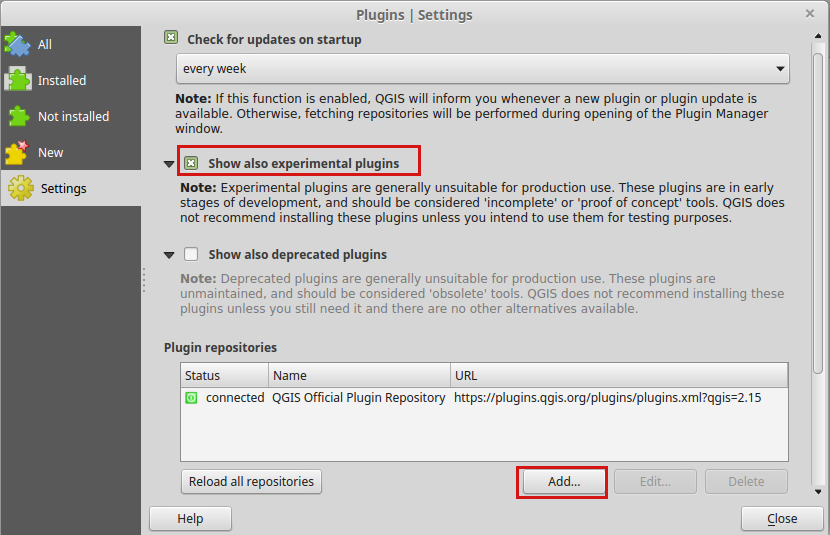
\includegraphics[width=1\textwidth]{images/qgis_repo_plugins.png}
\caption[Přidání repositáře QGIS]{Přidání repositáře QGIS}
\label{l_qgis_plugins}
\end{figure}

\begin{figure}[htb]
\centering
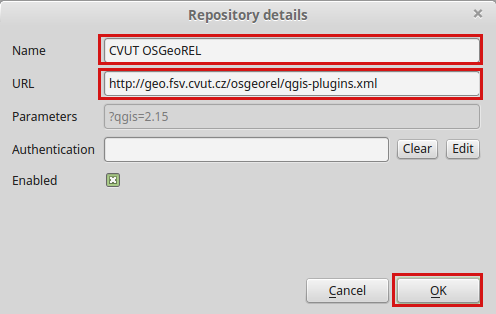
\includegraphics[width=0.5\textwidth]{images/qgis_repo_detail.png}
\caption[Přidání repositáře QGIS -- detail]{Přidání repositáře QGIS -- detail}
\label{l_repo_detail}
\end{figure}

Po přidání repositáře a~jeho aktualizaci je zásuvný modul dohledatelný
standardním způsobem pod názvem \textbf{VFK Plugin}, viz
obr. \ref{l_qgis_hledani_pluginu}.

\begin{figure}[htb]
\centering
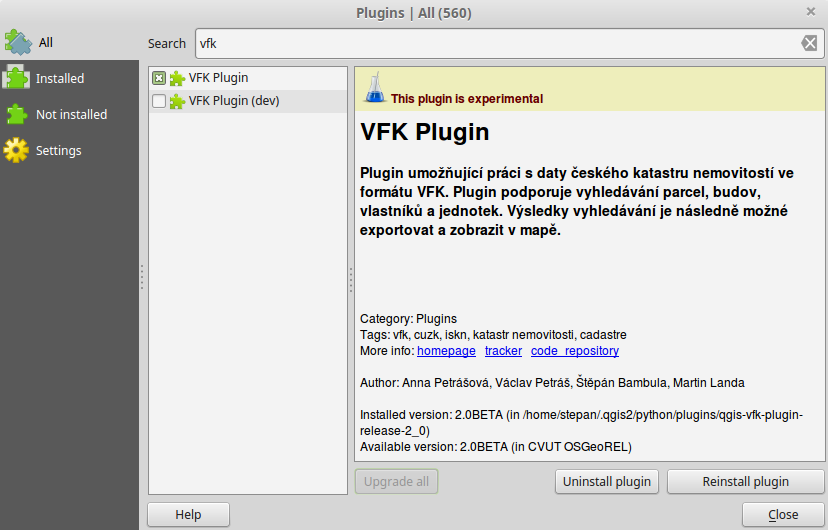
\includegraphics[width=1\textwidth]{images/qgis_plugin_vyhledani.png}
\caption[Vyhledání zásuvného modulu]{Vyhledání zásuvného modulu}
\label{l_qgis_hledani_pluginu}
\end{figure}

Po správné instalaci zásuvného modulu se do nástrojové lišty přidá
jeho ikonka (viz obr. \ref{l_plugin_ikona}). Plugin je poté dostupný
po kliknutí na tuto ikonku nebo z~menu \textit{Plugins} $\rightarrow$
\textit{VFK} $\rightarrow$ \textit{Otevřít prohlížeč VFK}.

\begin{figure}[H]
\centering

\includegraphics[scale=0.9]{images/vfkPluginIcon.png}
\caption[VFK Plugin -- ikona]{VFK Plugin -- ikona}
\label{l_plugin_ikona}
\end{figure}

Uživatelská přívětivost používání zásuvného modulu je zvýšena
\uv{dokovatelností} samotného okna pluginu. Modul je primárně ukotven
k~horní liště okna QGIS, ale je možné ho ukotvit i~k~ostatním
okrajům. Okno modulu lze samozřejmě používat i~samostatně
(neukotvené).

% -----------------------------------------------
\clearpage
\section{Rozložení zásuvného modulu}
Okno zásuvného modulu se skládá ze tří hlavních částí. Vlevo se
nachází hlavní panel nástrojů (obr \ref{l_plugin_prirucka_rozlozeni}
prvek č. 1) pro přepínání oken pro import souborů ve formátu
\textit{.vfk}, \textit{.db} a~pro vyhledávání. Naprostou většinu pravé
části tvoří prohlížeč dat (obr \ref{l_plugin_prirucka_rozlozeni} prvek
č. 2), ve kterém se zobrazují výsledky vyhledávání a~nápověda. Nad ním
je umístěna nástrojová lišta (obr \ref{l_plugin_prirucka_rozlozeni}
prvek č. 3), která obsahuje nástroje pro práci se zásuvným modulem.

\begin{figure}[H]
\centering
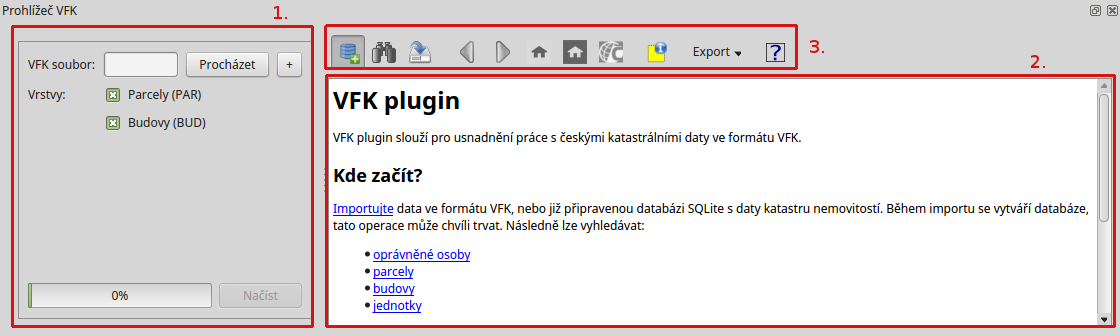
\includegraphics[width=1\textwidth]{images/vfkPlugin-prirucka_rozlozeni.png}
\caption[VFK Plugin -- rozložení prvků]{VFK Plugin -- rozložení prvků}
\label{l_plugin_prirucka_rozlozeni}
\end{figure}

% -----------------------------------------------
\section{Načítání dat}
Pomocí zásuvného modulu je možné nahrát soubor VFK nebo soubor
databáze SQLite, ve které jsou VFK data uložena. Tento import je
k~dispozici pomocí tlačítka \uv{Procházet} v~nabídce \textit{Import
  VFK}.

Zásuvný modul podporuje načítání více souborů. Formulář pro načtení
dalšího VFK souboru je vygenerován po stisku tlačítka \uv{+}. Cesta
k~novému souboru se zadává opět po stisku tlačítka \uv{Procházet}.

V~tomto okně je dále možné zvolit, které vrstvy se budou importovat
(PAR, BUD). V~případě, kdy není zatrženo ani jedno pole, tak se načtou
pouze popisná data. Bude tedy dostupné pouze vyhledávání bez interakce
s~mapovým oknem.

Jestliže je na vstupu zadán soubor ve formátu \textit{.vfk}, tak je na
pozadí vytvořená databáze SQLite, do které jsou data z~VFK souboru
načteny. Tato databáze je pojmenována
\texttt{jmeno\_prvniho\_souboru\_stav.db} pro případ, kdy načtený
soubor obsahuje stavová data, nebo
\texttt{jmeno\_prvniho\_souboru\_zmeny.db}, když jsou v~prvním souboru
uložena změnová data. Databáze je uložena o~adresář výše, než první
soubor VFK.

Funkcionalita pro načítání více souborů a~načítání dat z~SQLite
databáze je do zásuvného modulu přidána pouze v~případě, kdy je na
počítači uživatele dostupná knihovna GDAL ve verzi \texttt{2.2.0}
a~vyšší.

% -----------------------------------------------
\section{Vyhledávání}
Po úspěšném načtení dat je zpřístupněno vyhledávání. Výsledky
vyhledávání se zobrazují ve vedlejším okně, prohlížeči dat. Tato data
lze interaktivně procházet, podobně jako je tomu ve webovém
prohlížeči, jelikož jsou ukládána ve formě HTML stránek. Pro navigaci
mezi jednotlivými prvky jsou používány hypertextové odkazy. Obsah okna
prohlížeče je ukládán do historie, což usnadňuje uživateli vyhledávání
stále se opakujících informací (není potřeba opakovaně provádět stejný
databázový dotaz). Historii lze procházet pomocí tlačítek \uv{Vpřed}
a~\uv{Zpět}.

Pro zjištění aktuálního stavu o~dané nemovitosti je zde implementováno
propojení s~aplikací \textbf{Nahlížení do katastru
  nemovitostí}\footnote{http://nahlizenidokn.cuzk.cz/}.

Zásuvný modul a~mapové okno QGIS jsou navzájem propojené. Je tedy
možné v~mapovém okně zobrazit polohu vyhledaných prvků a~opačně
vyhledat informace o~prvcích, které byly vybrány pomocí nástroje
výběru QGIS právě v~mapovém okně (při výběru prvků z~mapového okna je
potřeba aktivovat tlačítko \uv{Aktivovat / deaktivovat zobrazení
  informací o~vybraných nemovitostech}).

Vyhledávat lze podle následujících prvků:

\begin{itemize}
 \item vlastníků,
 \item parcel,
 \item budov,
 \item jednotek.
\end{itemize}

\begin{figure}[htb]
    \centering
    \begin{subfigure}[b]{0.4\textwidth}
        \centering
        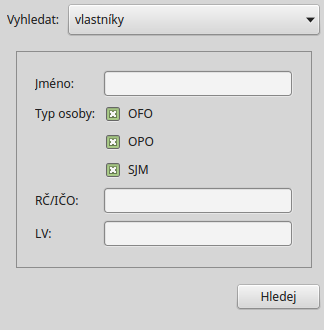
\includegraphics[width=\textwidth]{images/vfkPlugin-vlastnici.png}
        \caption{Vyhledávání vlastníků}
    \end{subfigure}
    ~
    \begin{subfigure}[b]{0.4\textwidth}
        \centering
        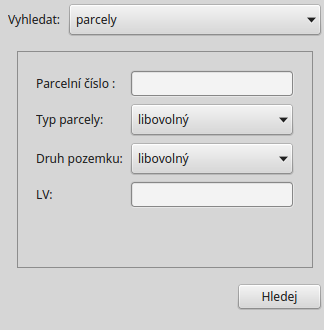
\includegraphics[width=\textwidth]{images/vfkPlugin-parcely.png}
        \caption{Vyhledávání parcel}
    \end{subfigure}
    \caption{Vyhledávací formuláře 1/2}
    \label{l_vyhledavani_1}
\end{figure}

\begin{figure}[htb]
    \centering
    \begin{subfigure}[b]{0.393\textwidth}
        \centering
        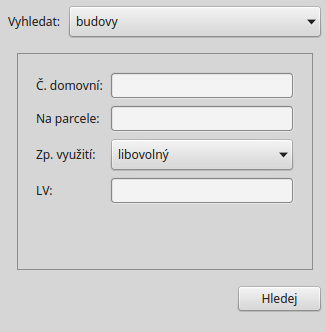
\includegraphics[width=\textwidth]{images/vfkPlugin-budovy.png}
        \caption{Vyhledávání budov}
    \end{subfigure}
    ~
    \begin{subfigure}[b]{0.4\textwidth}
        \centering
        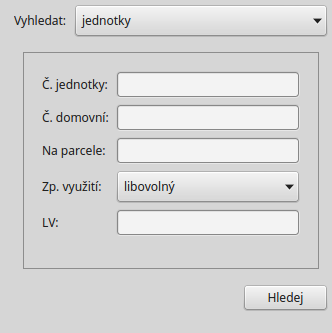
\includegraphics[width=\textwidth]{images/vfkPlugin-jednotky.png}
        \caption{Vyhledávání jednotek}
    \end{subfigure}
    \caption{Vyhledávací formuláře 2/2}
    \label{l_vyhledavani_1}
\end{figure}


\clearpage
% -----------------------------------------------
\section{Export vyhledaných informací}
Veškeré vyhledané informace, které jsou zobrazeny v~prohlížeči dat, je
možné uložit. Export může být proveden do souboru v~následujících
formátech:

\begin{itemize}
\item \textbf{HTML}: Umožňuje následné zobrazení ve webovém
  prohlížeči, případně import do textového procesoru
 \item \textbf{Zdrojový kód \latex}: Umožňuje vytvoření PDF nebo PS.
\end{itemize}

% -----------------------------------------------
\section{Zpracování změn}
Funkcionalita pro zpracování změn je dostupná pod příslušnou ikonou
(obr \ref{l_ikona_zmen}). Po stisku této ikony je vygenerováno nové
okno s~následujícími prvky:

\begin{figure}[htb]
\centering

\includegraphics[scale=0.9]{images/applyChanges.png}
\caption[VFK Plugin -- ikona pro zpracování změn]{VFK Plugin -- ikona pro zpracování změn}
\label{l_ikona_zmen}
\end{figure} 

\begin{enumerate} 
\item \textbf{Formuláře:} K~dispozici jsou tři formuláře pro zadání
  cesty ke vstupní databázi se stavovými daty, k~databázi se změnovými
  daty a~databázi výstupní, do které budou uložena stavová data
  s~aplikovanými změnami.
 
\item \textbf{Popisek průběhu zpracování:} V~tomto popisku jsou
  zobrazovány informace o~průběhu zpracování změn.
 
\item \textbf{Grafický indikátor průběhu:} Zde je průběh zpracování
  změn vyjádřen procentuálně a~graficky.
 
\item \textbf{Tlačítko pro zpracování:} Po stisku tohoto tlačítka jsou
  změny aplikovány do databáze se stavovými daty.
 
\end{enumerate}

\begin{figure}[htb]
\centering
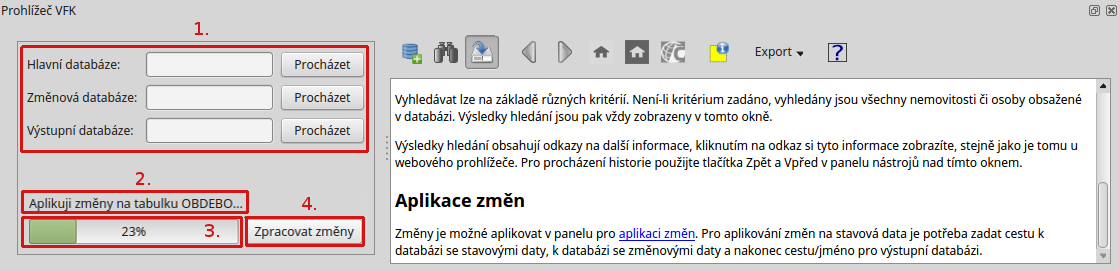
\includegraphics[width=0.9\textwidth]{images/vfkPlugin-prirucka_zmeny.png}
\caption[VFK Plugin -- okno pro zpracování změn]{VFK Plugin -- okno pro zpracování změn}
\label{l_plugin_zmeny}
\end{figure}

Postup zpracování změn je následující. Nejprve jsou načteny pomocí
tlačítek \uv{Procházet} databáze se stavovými daty a~databáze se
změnami. Dále je potřeba zadat cestu k~nově vytvořené databázi, do
které budou změny aplikovány. Po zadání těchto informací je
zpřístupněno tlačítko \uv{Zpracovat změny}. Změny jsou na stavová data
aplikovány po jeho stisknutí.

Funkcionalita pro aplikaci změn obsažených v~databázi SQLite na data
obsažená v~databázi se stavovými daty je do zásuvného modulu přidána
pouze v~případě, kdy je na počítači uživatele dostupná knihovna GDAL
ve verzi \texttt{2.2.0} a~vyšší. V~opačném případě je ikonka pro
zpracování změn neaktivní.

%-----------------------------------------------
\chapter{Obsah přiloženého CD}

\begin{enumerate}
 \item Zdrojové kódy zásuvného modulu.
 \item Patch knihovny GDAL ve verzi 2.2.0.
\end{enumerate}



\end{document}
